\documentclass[journal]{IEEEtran}

% *** CITATION PACKAGES ***
\usepackage{cite}

% *** GRAPHICS RELATED PACKAGES ***
\usepackage{graphicx}

% *** MATH PACKAGES ***
\usepackage{amsmath,amssymb,amsfonts}

% *** OTHER USEFUL PACKAGES ***
\usepackage{stfloats}
\usepackage{url}
\usepackage{hyperref}
\usepackage{comment}
\usepackage{tikz}
\usepackage{pgfplots}
\usepgfplotslibrary{groupplots}
\pgfplotsset{compat=1.18}
\usetikzlibrary{
  arrows.meta,
  shapes.geometric,
  positioning,
  fit,
  calc,
  backgrounds,
  shadows,
  patterns,
  matrix,
  decorations.pathreplacing
}


\definecolor{ieee_blue}{RGB}{0, 98, 155}
\definecolor{ieee_red}{RGB}{180, 0, 30}
\definecolor{soft_gray}{RGB}{240, 240, 240}
\definecolor{dark_gray}{RGB}{60, 60, 60}
\definecolor{ieee_orange}{RGB}{255, 127, 0}
\definecolor{ieee_green}{RGB}{0, 128, 0}
\definecolor{forest_green}{RGB}{34, 139, 34}
\definecolor{saturation_gray}{RGB}{220, 220, 220}
\definecolor{budget_red}{RGB}{220, 20, 60}
\definecolor{stage_blue}{RGB}{225, 240, 255} % Lighter for better contrast
\definecolor{stage_green}{RGB}{225, 255, 225}
\definecolor{stage_orange}{RGB}{255, 240, 220}
\definecolor{invariant_purple}{RGB}{147, 112, 219}
\definecolor{hw_gray}{RGB}{80, 80, 80}
\definecolor{border_gray}{RGB}{120, 120, 120}



% Colors matched to manuscript description
\definecolor{local_blue}{RGB}{0, 114, 189}    % "samplers compute local posteriors (blue)"
\definecolor{shared_green}{RGB}{119, 172, 48} % "aggregated into shared beliefs (green)"
\definecolor{process_gray}{RGB}{240, 240, 240}
\definecolor{signal_red}{RGB}{162, 20, 47}

% Professional Color Palette
\definecolor{k8s_blue}{RGB}{50, 108, 229}      % Kubernetes
\definecolor{control_purple}{RGB}{102, 51, 153} % IBG Controller
\definecolor{pod_green}{RGB}{46, 139, 87}       % Kernel App
\definecolor{dpdk_orange}{RGB}{255, 140, 0}     % DPDK App
\definecolor{net_gray}{RGB}{80, 80, 80}         % Network/Hardware
\definecolor{alert_red}{RGB}{220, 20, 60}       % Constraints/Emulation

% Professional Colors
\definecolor{proc_blue}{RGB}{0, 114, 189}
\definecolor{data_green}{RGB}{119, 172, 48}
\definecolor{infra_gray}{RGB}{128, 128, 128}
\definecolor{highlight_gray}{RGB}{240, 240, 240}

% IEEE Colors
\definecolor{ieee_green}{RGB}{0, 128, 0}
\definecolor{ieee_orange}{RGB}{255, 127, 0}
\definecolor{dark_gray}{RGB}{80, 80, 80}



% Declare layers to ensure background strictly stays behind
\pgfdeclarelayer{background}
\pgfsetlayers{background,main}

% Declare layers to ensure background boxes are actually behind the nodes
\pgfdeclarelayer{background}
\pgfsetlayers{background,main}


% *** THEOREM ENVIRONMENTS ***
\usepackage{amsthm}
\theoremstyle{plain}
\newtheorem{theorem}{Theorem}
\newtheorem{proposition}{Proposition}
\newtheorem{corollary}{Corollary}
\newtheorem{lemma}{Lemma}[section]

\theoremstyle{definition}
\newtheorem{definition}{Definition}
\newtheorem{assumption}{Assumption}

\theoremstyle{remark}
\newtheorem{remark}{Remark}

% *** ALGORITHM PACKAGE (choose ONE) ***
% Use algorithm2e OR algorithmicx, not both
\usepackage[ruled,vlined,linesnumbered]{algorithm2e}
% If you prefer pseudocode instead, comment the above line and use the next two:
% \usepackage{algorithm}
% \usepackage{algpseudocode}

% correct bad hyphenation here
\hyphenation{op-tical net-works semi-conduc-tor}


\begin{document}

\title{Learning to Chain: An Indian-Buffet-Game Approach for Distributed Service Function Chaining in Containerized 6G Cores}

\author{???~???~\IEEEmembership{}
        and~Vesal~Hakami~\IEEEmembership{}% <-this % stops a space
\thanks{???. ??? is with the School of Computer Engineering, Iran University of Science and Technology (IUST), Tehran, Iran.}
\thanks{Corresponding author: V. Hakami (e-mail: vhakami@iust.ac.ir; URL: \url{http://webpages.iust.ac.ir/vhakami}). Postal address: Center of Excellence in Future Networks, School of Computer Engineering, Iran University of Science and Technology (IUST), Tehran 16846-13114, Iran. Tel: +98-(21)73225326.}}


% The paper headers
\markboth{IEEE Transactions on Network Systems and Management,~Vol.~XX, No.~X, August~2025}%
{Hakami \MakeLowercase{\textit{et al.}}: IBG 6G Core SFC}


% make the title area
\maketitle


\begin{abstract}
Cloud-native 6G cores require distributed, privacy-aware mechanisms for Service Function Chain (SFC) placement across containerized network functions (CNFs) under tenant-specific QoS constraints. We model this as an Indian Buffet Game (IBG), a sequential game with incomplete information, where tenant flows choose CNF replicas for each NF stage (e.g., AMF, SMF, UPF) while contending for resources. Each replica has an unknown latent state (host load, interference, acceleration mode), and only flows traversing a replica observe its performance signal. To address asymmetric telemetry, we embed a non-Bayesian social learning rule that combines local Bayesian posteriors via lightweight aggregation, proving weak convergence of predictive marginals. Under a no cross-stage coupling assumption, we present an exact backward-induction algorithm (\textsf{BR\_EIBG}) that constructs subgame-perfect Nash equilibria (SPNE). For the general coupled setting, we prove the intractability of the exact solution and design a \textbf{scalable hybrid pipeline} that composes candidate pruning with limited-lookahead rollouts. This approach reduces decision complexity from exponential to polynomial while preserving strategic foresight. Our contributions include the formal IBG–SFC mapping, convergence analysis, and a Kubernetes/NSM implementation blueprint. Simulations show our hybrid approach achieves near-centralized utility (within 2\%), reduces SLA violations by $>$50\%, and cuts control-plane overhead by 10$\times$ versus MILP/DRL baselines, demonstrating viability for real-time 6G admission control.
\end{abstract}

\begin{IEEEkeywords}
???
\end{IEEEkeywords}

\section{Introduction}\label{sec:intro}

\subsection{Motivation and Problem Statement}
\label{sec:intro_motivation}

The evolution toward cloud-native 6G core networks necessitates a fundamental rethinking of Service Function Chaining (SFC) orchestration. Network functions are now deployed as ephemeral, containerized microservices (CNFs) managed by Kubernetes, enabling rapid elasticity but introducing significant operational complexity for distributed SFC placement. A critical challenge is to map sequential tenant flows to concrete CNF replicas (pods) across an ordered chain of stages (e.g., AMF, SMF, UPF) while simultaneously satisfying stringent per-flow QoS requirements and optimizing system-wide resource efficiency.

This problem is inherently difficult due to three intertwined factors. First, CNF replica performance is highly uncertain and time-varying, governed by latent host conditions such as background CPU load, noisy co-tenant interference, and the state of data-plane acceleration (e.g., VPP/DPDK vs. kernel path) []. Second, performance observations are fundamentally asymmetric: only flows routed through a specific replica can directly observe its instantaneous quality (e.g., processing delay, packet loss); other flows and the orchestrator receive no raw telemetry, primarily for privacy and scalability reasons []. Third, placement decisions are sequential and induce negative network externalities: as more flows select the same replica, the utility for each degrades due to resource contention, meaning early assignments directly impact the feasible choices and welfare of subsequent flows [].

Consequently, a practical SFC placement mechanism for 6G cores must operate in a distributed, online fashion, making decisions under uncertainty while accounting for strategic interactions and respecting strict control-plane bandwidth budgets. Centralized, clairvoyant optimization is infeasible at operational scale, and naive heuristics that ignore either the learning or strategic aspects lead to suboptimal global performance and unfairness. This paper addresses this challenge by formulating SFC placement as a sequential game of incomplete information, where flows learn and act strategically in a shared, uncertain environment.

\subsection{Limitations of Existing Approaches}
\label{sec:intro_limitations}

Existing literature offers diverse solutions for SFC placement, yet significant limitations persist, particularly in addressing the unique challenges of cloud-native 6G environments. These shortcomings can be categorized into three main areas.

First, centralized optimization frameworks, typically based on Mixed-Integer Linear Programming (MILP), provide optimal benchmarks but suffer from prohibitive computational complexity [1], [2]. This renders them intractable for the dynamic, large-scale scenarios characteristic of 6G cores. Furthermore, these models presuppose perfect and instantaneous knowledge of replica performance, an assumption that is fundamentally violated in practice due to latent states and asymmetric observability.

Second, learning-based approaches, particularly Deep Reinforcement Learning (DRL), have emerged as a scalable alternative [3], [4]. However, DRL agents are often sample-inefficient, requiring extensive training to converge, and their "black-box" policies lack interpretability, complicating operational debugging and trust. Critically, most single-agent or multi-agent DRL formulations treat the environment as stationary, failing to model the strategic interdependence where one flow's decision directly impacts the utility of others.

Third, game-theoretic models, such as congestion games and auction mechanisms, elegantly capture strategic behavior [5], [6]. Their primary drawback in this context is the pervasive assumption of common knowledge regarding resource qualities and payoffs. These models typically assume all players (flows) have a priori knowledge of replica performance distributions, which sidesteps the core learning problem under asymmetric information. Moreover, reaching equilibrium often entails significant inter-agent communication, challenging low-overhead requirements.

In summary, prior models address isolated aspects of the problem—optimization for efficiency, learning for uncertainty, or game theory for contention—but lack an integrated framework that unifies distributed decision-making, online learning under asymmetric information, and negative network externalities. This gap motivates the development of a game-theoretic and learning-driven approach specifically tailored to containerized 6G core environments.

\subsection{Our Approach and Key Contributions}
\label{sec:intro_contributions}

This paper introduces a novel framework that models distributed SFC placement in cloud-native 6G cores as an Indian Buffet Game (IBG). This formulation naturally captures the sequential arrival of tenant flows, their strategic selection of CNF replicas, and the negative externalities induced by resource contention. To handle the inherent uncertainty in replica performance and the challenge of asymmetric observations, we employ a lightweight, non-Bayesian social learning rule where flows update their beliefs based on local signals and aggregate posterior summaries.

Our primary contributions are fourfold:
\begin{itemize}
    \item \textbf{IBG Formulation for SFC:} We are the first to formally map the distributed SFC placement problem to an IBG, providing a rigorous game-theoretic foundation for modeling sequential, strategic replica selection under uncertainty.
    
    \item \textbf{Distributed Learning under Asymmetry:} We design a practical non-Bayesian social learning rule that enables flows to collaboratively infer latent replica states with minimal control-plane overhead, respecting privacy constraints by avoiding raw data sharing. We prove its predictive marginals converge to the true performance distribution.
    
    \item \textbf{Exact Algorithms and Hybrid Pipeline:} We develop exact, recursive best-response algorithms (\textsf{BR\_EIBG}, \textsf{BR\_IBG}) to characterize the theoretical SPNE. To address the NP-hardness arising from \textbf{cross-stage resource dependencies} (e.g., shared budgets and link latencies), we design a \textbf{Hybrid Decision Pipeline} that structurally pipelines candidate pruning with limited-lookahead rollouts. This composition reduces decision complexity from exponential to polynomial, making game-theoretic orchestration tractable for large-scale systems.
    
    \item \textbf{Systems Implementation and Validation:} We provide a practical implementation blueprint using Kubernetes sidecars. Extensive experiments on a hybrid testbed demonstrate that our pipeline achieves near-optimal utility (within 2\% of MILP), reduces SLA violations by $>$50\%, and cuts control-plane overhead by 10$\times$ versus DRL baselines, validating its suitability for real-time 6G admission control.
\end{itemize}

\subsection{Paper Organization}
\label{sec:intro_organization}

The remainder of this paper is organized as follows. Section II reviews related work. Section III presents the system model and problem formulation. Section IV details our IBG-based framework for SFC. Section V describes the exact SPNE algorithms, while Section VI introduces our suite of scalable approximations for practical deployment. Section VII details the distributed learning rule and its convergence properties. Section VIII provides a comprehensive experimental evaluation of our proposed algorithms. Finally, Section IX concludes the paper. 

\begin{table}[!t]
\centering
\caption{List of Key Acronyms}
\label{tab:acronyms}
\renewcommand{\arraystretch}{1.2}
\begin{tabular}{l l}
\toprule
\textbf{Acronym} & \textbf{Definition} \\
\midrule
6G & Sixth Generation Mobile Networks \\
AMF & Access and Mobility Management Function \\
CNF & Containerized Network Function \\
DPDK & Data Plane Development Kit \\
DRL & Deep Reinforcement Learning \\
IBG & Indian Buffet Game \\
MILP & Mixed-Integer Linear Programming \\
NSM & Network Service Mesh \\
QoS & Quality of Service \\
SFC & Service Function Chaining \\
SLA & Service Level Agreement \\
SMF & Session Management Function \\
SPNE & Subgame-Perfect Nash Equilibrium \\
UPF & User Plane Function \\
VPP & Vector Packet Processing \\
URLLC & Ultra-Reliable Low-Latency Communication \\
\bottomrule
\end{tabular}
\end{table}


\section{Related Work}
\label{sec:related_work}

The placement and chaining of network functions have been extensively studied in network virtualization. However, the transition from Virtual Network Functions (VNFs) on virtual machines to lightweight Containerized Network Functions (CNFs) in 6G core networks has introduced a new class of scalability, observability, and privacy challenges. Classical approaches, designed for static and homogeneous VNFs, do not readily extend to the dynamic, fine-grained, and privacy-sensitive nature of cloud-native cores. To contextualize this work, we first establish a concise analytical framework of key taxonomical perspectives and evaluation criteria that guide the subsequent review.

\subsection{Taxonomical Perspectives and Evaluation Criteria}

Prior research on Service Function Chaining (SFC) and resource allocation can be categorized by several fundamental dimensions that determine scalability, adaptability, and realism of information assumptions.

\textbf{Control Architecture (Centralized vs.\ Distributed):}
Centralized frameworks rely on a logically global controller that maintains complete knowledge of the network topology, resource capacities, and traffic demands []. They commonly employ Mixed‑Integer Linear Programming (MILP) or constraint‑programming formulations to derive globally optimal placements []. While offering optimal benchmarks, these methods impose heavy computational and signaling overheads and are unsuitable for real‑time admission control at 6G scale. Distributed approaches delegate decisions to multiple autonomous agents operating with only local information []. Such schemes, including heuristic and game‑theoretic methods, improve scalability and fault tolerance but must coordinate efficiently to approach near‑optimal system‑wide performance without centralized synchronization.

\textbf{Implementation Paradigm (VNF‑based vs.\ CNF‑based):}
Earlier SFC research focused on VNFs—monolithic functions hosted on virtual machines—where performance is relatively static and predictable []. In contrast, CNFs are microservice‑based and orchestrated by platforms such as Kubernetes. They are ephemeral, rapidly scalable, and highly heterogeneous due to host‑level noise and data‑plane acceleration (e.g., VPP/DPDK) []. Conventional VNF placement algorithms thus fail to capture the elasticity and stochastic performance variations characteristic of CNFs.

\textbf{System‑State Modeling (Deterministic vs.\ Stochastic):}
Deterministic models assume each instance’s processing capacity and latency are fixed and known [], simplifying optimization but neglecting time‑varying host conditions, NUMA interference, and multiplexing dynamics. Stochastic formulations, often leveraging Reinforcement Learning (RL) or Multi‑Armed Bandit (MAB) frameworks [], explicitly model uncertainty and learn instance performance online. The proposed work builds on this stochastic perspective but further incorporates latent states and asymmetric observability, which are essential for privacy‑aware telemetry.

\textbf{Decision Timing and Granularity (Offline vs.\ Online):}
Offline algorithms compute placements for batches of requests with full a‑priori information, suitable only for static or long‑lived services []. Online algorithms decide sequentially as flows arrive, reacting to evolving conditions without knowledge of future demands []. This online, sequential setting is the operative regime in 6G systems and gives rise to strategic externalities as early placements affect the utilities of subsequent arrivals.

\textbf{Evaluation Criteria:}
Building on these dimensions, we assess approaches according to four criteria:
(i)~\emph{Scalability and Control‑Plane Overhead}—how complexity and signaling grow with network size;  
(ii)~\emph{Informational Realism and Privacy}—whether full system telemetry or only partial, privacy‑filtered views are assumed;  
(iii)~\emph{Solution Quality and Guarantees}—optimality, convergence, or equilibrium stability; and  
(iv)~\emph{Adaptability and Robustness}—the ability to maintain high performance under CNF churn, dynamic traffic, and shifting load conditions.

This taxonomy provides the basis for a concise evaluation of existing SFC placement methods in the following subsections.

\subsection{Literature Review}
\label{sec:related_litreview}

Following the aforementioned taxonomy, prior work on SFC placement can be grouped into three main categories: centralized optimization, learning‑based orchestration, and distributed game‑theoretic or multi‑agent systems. Each offers valuable insights but falls short of addressing the combined challenges of uncertainty, sequential decision‑making, and privacy‑constrained observability in containerized 6G cores.

\textbf{Centralized Exact and Heuristic Approaches:}
Early studies modeled VNF placement as a global optimization problem, typically using Mixed‑Integer Linear Programming (MILP) or Integer Linear Programming (ILP) to minimize cost, latency, or energy consumption []. These formulations provide exact baselines but are NP‑hard and computationally infeasible for networks with thousands of replicas and real‑time flow arrivals. The reliance on global, static state information further renders them unsuitable for dynamic CNF environments. To mitigate complexity, numerous heuristics—First‑Fit, Best‑Fit, latency‑aware greedy algorithms, and resource‑balancing strategies—have been proposed []. Such methods achieve faster decisions but remain myopic, optimizing only immediate requests and ignoring the long‑term effects of congestion and flow interactions, which leads to fragmented resource usage and degraded global utility.

\textbf{Centralized Learning‑Based Approaches:}
More recent works employ Machine Learning (ML), particularly Deep Reinforcement Learning (DRL), to handle stochastic and time‑varying network conditions []. In these frameworks, a central agent learns a mapping from global network states to placement actions to minimize SLA violations or routing costs []. Techniques such as Deep‑Q Networks (DQN), Actor–Critic models, and Graph Neural Networks (GNNs) have been explored to improve scalability and exploit network topology features []. Although effective in simulation, these approaches depend on a centralized controller with global visibility and full telemetry access, creating both performance bottlenecks and privacy concerns in multi‑tenant 6G infrastructures. Their opaque policies also hinder interpretability and lack provable guarantees of fairness or stability. Multi‑Armed Bandit formulations offer lighter alternatives for online server or path selection [], but they generally neglect correlations among concurrent flow decisions and ignore contention‑induced externalities.

\textbf{Distributed Game‑Theoretic and Multi‑Agent Models:}
To overcome central bottlenecks, distributed schemes model interactions among tenants or flows as strategic games []. Auction‑based mechanisms and Stackelberg games have been proposed for resource allocation and pricing [], while congestion games describe load‑dependent utility degradation due to shared resource usage []. These models capture competition and coordination but typically assume complete or symmetric information—each player knows the utility or quality of all resources—which is unrealistic when CNF performance is latent and observable only to users of that replica. Moreover, most formulations treat the system as static or simultaneous‑move, omitting the sequential nature of flow admissions that gives rise to dynamic externalities. Only a few recent studies combine distributed coordination with online learning, but they still assume shared information or unrestricted telemetry exchange [].  

\subsection{Positioning Our Work}
\label{sec:related_positioning}

The preceding review highlights that current research addresses individual facets of the SFC placement problem but fails to provide an integrated, analytically grounded solution that reflects the realities of cloud‑native 6G cores. Centralized optimizers offer optimal benchmarks yet cannot scale to thousands of ephemeral CNFs or operate with limited telemetry. Learning‑based controllers adapt to stochastic performance but rely on centralized visibility and black‑box policies with no formal stability guarantees. Distributed game‑theoretic approaches elegantly capture resource contention but generally presume complete information, neglecting the need to infer unknown replica performance from partial, privacy‑filtered observations.  

Our work bridges these disjoint lines of research through a unified, game‑theoretic and learning‑driven framework. By casting SFC placement as an Indian Buffet Game, we explicitly model sequential flow arrivals, latent CNF states, and negative network externalities within a single formalism.

\section{System Model and Problem Formulation}
\label{sec:sys_model}

\subsection{Network and Service Model}
\label{sec:sys_network}

\begin{table}[!t]
\centering
\caption{Summary of Important Notations}
\label{tab:notations}
\renewcommand{\arraystretch}{1.2}
\begin{tabular}{l p{6cm}}
\toprule
\textbf{Symbol} & \textbf{Definition} \\
\midrule
\multicolumn{2}{c}{\textit{System and Network Model}} \\
\midrule
$\mathcal{N}, N$ & Set of tenant flows $\{1,\dots,N\}$ arriving in a slot \\
$\mathcal{T}, K$ & Set of SFC stages $\{1,\dots,K\}$ \\
$\mathcal{I}_k, M_k$ & Set of replicas available at stage $k$ \\
$\mathcal{H}$ & Set of physical/Kubernetes nodes \\
$\mathbf{C}_h$ & Resource capacity vector of node $h$ \\
$\kappa_{k,j}$ & Baseline processing capacity of replica $(k,j)$ \\
$a_{k,j}^{(t)}$ & Binary availability state of replica $(k,j)$ in slot $t$ \\
$\pi^{(t)}$ & Random arrival permutation of flows in slot $t$ \\
\midrule
\multicolumn{2}{c}{\textit{Game and Decision Variables}} \\
\midrule
$d_{i,k,j}^{(t)}$ & Binary decision: 1 if flow $i$ selects replica $(k,j)$ \\
$\mathbf{d}_i$ & Placement strategy vector/path for flow $i$ \\
$N_{k,j}^{(t)}$ & Final load (number of flows) on replica $(k,j)$ \\
$n_{k,j}^{(t)}$ & Pre-decision count (observed by flow $i$ before acting) \\
$U_i^{(t)}$ & Total expected utility of flow $i$ \\
$u_k(q,n)$ & Per-stage utility kernel (quality $q$, load $n$) \\
\midrule
\multicolumn{2}{c}{\textit{Learning and Uncertainty}} \\
\midrule
$\theta_{k,j}$ & Latent performance state (e.g., Load, Interference) \\
$\Theta$ & Finite set of possible latent states \\
$s_{i,k,j}^{(t)}$ & Private performance signal observed by flow $i$ \\
$f(\cdot|\theta)$ & Likelihood function of signal given state $\theta$ \\
$p_{k,j}^{(t)}(\theta)$ & Belief probability that replica $(k,j)$ is in state $\theta$ \\
$\mu_{i,k,j}^{(t)}$ & Local Bayesian posterior computed by flow $i$ \\
$\lambda_{k,j}^{(t)}(s)$ & Predictive marginal distribution of signals \\
\midrule
\multicolumn{2}{c}{\textit{Approximation Algorithms}} \\
\midrule
$\Phi$ & Full set of feasible placement combinations \\
$\Phi_C$ & Pruned set of top-$C$ candidate paths \\
$C$ & Candidate pruning size (Pipeline Stage 1) \\
$D$ & Lookahead depth (Pipeline Stage 2) \\
$S$ & Number of Monte Carlo samples (Pipeline Stage 3) \\
\bottomrule
\end{tabular}
\end{table}

We consider a cloud‑native 6G core network in which network functions are implemented as \emph{Containerized Network Functions} (CNFs) orchestrated by Kubernetes. Each core function type—such as the Access and Mobility Management Function (AMF), Session Management Function (SMF), User Plane Function (UPF), and Policy Control Function (PCF)—is represented by a set of concurrently active \emph{replicas} (pods) hosted on a pool of compute nodes. The set of nodes is denoted by $\mathcal{H}=\{1,\dots,H\}$, and each node $h\in\mathcal{H}$ offers finite processing, memory, and bandwidth capacities $\mathbf{C}_h=(C_h^{\mathrm{cpu}},C_h^{\mathrm{mem}},C_h^{\mathrm{bw}})$.

Let $\mathcal{T}=\{1,\dots,K\}$ denote the ordered set of service chain stages. Each stage $k\in\mathcal{T}$ hosts $M_k$ concurrently available CNF replicas indexed by $\mathcal{I}_k=\{1,\dots,M_k\}$. The $(k,j)$‑th replica, representing the $j$‑th instance of function type $k$, runs on node $h(k,j)\in\mathcal{H}$ and declares a resource‑request vector $\boldsymbol{\rho}_{k,j}=(\rho_{k,j}^{\mathrm{cpu}},\rho_{k,j}^{\mathrm{mem}}, \rho_{k,j}^{\mathrm{bw}})$. A placement is feasible only if, for every node $h$, the aggregated requested resources of all replicas scheduled on $h$ do not exceed $\mathbf{C}_h$.

We model the set of replicas belonging to all stages as $\mathcal{I}=\bigcup_{k=1}^{K}\{(k,j):j\in\mathcal{I}_k\}$. Replica $(k,j)$ may differ in implementation or acceleration mode; for example, $\iota_{k,j}\in\{\text{DPDK},\text{Kernel}\}$ specifies whether the instance uses a high‑performance user‑space data plane or the kernel path, with a baseline capacity parameter $\kappa_{k,j}$ representing its nominal processing capability.

Each decision epoch (slot) admits a batch of $N$ new flows, $\mathcal{N}=\{1,\dots,N\}$, that require SFC traversal through all $K$ stages. Flows arrive sequentially during the slot in a random order $\pi^{(t)}$, reflecting session establishment in practical systems. When served, flow $i$ selects exactly one replica per stage; the binary decision variable
\begin{equation}
d^{(t)}_{i,k,j}=
\begin{cases}
1,& \text{if flow }i\text{ uses replica }(k,j)\text{ at stage }k,\\
0,& \text{otherwise,}
\end{cases}
\label{eq:decision_variable}
\end{equation}
encodes its placement choice in time slot $t$. Feasibility requires
\begin{equation}
\sum_{j\in\mathcal{I}_k} d^{(t)}_{i,k,j}=1,\qquad 
\forall i\in\mathcal{N},\; \forall k\in\mathcal{T}.
\label{eq:one_per_stage}
\end{equation}
The number of flows sharing replica $(k,j)$ in slot $t$ is denoted
\begin{equation}
N^{(t)}_{k,j}=\sum_{i=1}^{N} d^{(t)}_{i,k,j}.
\label{eq:replica_load}
\end{equation}

For realism, each flow can observe the previous placements within the current slot; early assignments are visible as pre‑decision counts
$n_{k,j}^{(t)}(m-1)=\sum_{\ell=1}^{m-1} d^{(t)}_{\pi^{(t)}(\ell),k,j}$.
This sequential model mirrors practical admission‑control procedures where earlier flows influence later ones through emerging congestion.

Replica availability is represented by the binary state $a_{k,j}^{(t)}\!\in\!\{0,1\}$, where $a_{k,j}^{(t)}\!=\!1$ indicates availability during slot~$t$, reflecting failures or scaling events. The active set is $\mathcal{I}^{(t)}=\{(k,j)\in\mathcal{I} : a_{k,j}^{(t)}=1\}$, and decisions must satisfy $d_{i,k,j}^{(t)}\!\le\! a_{k,j}^{(t)}$ for feasibility.

The timescale of the decision epoch is chosen consistent with operational control loops in 6G orchestration (hundreds of milliseconds), allowing replica states to remain approximately stationary within a slot while enabling fast reconfiguration across slots.

\begin{figure*}[h!] 
\centering
% Resize the entire TikZ picture to the full text width
\resizebox{\textwidth}{!}{
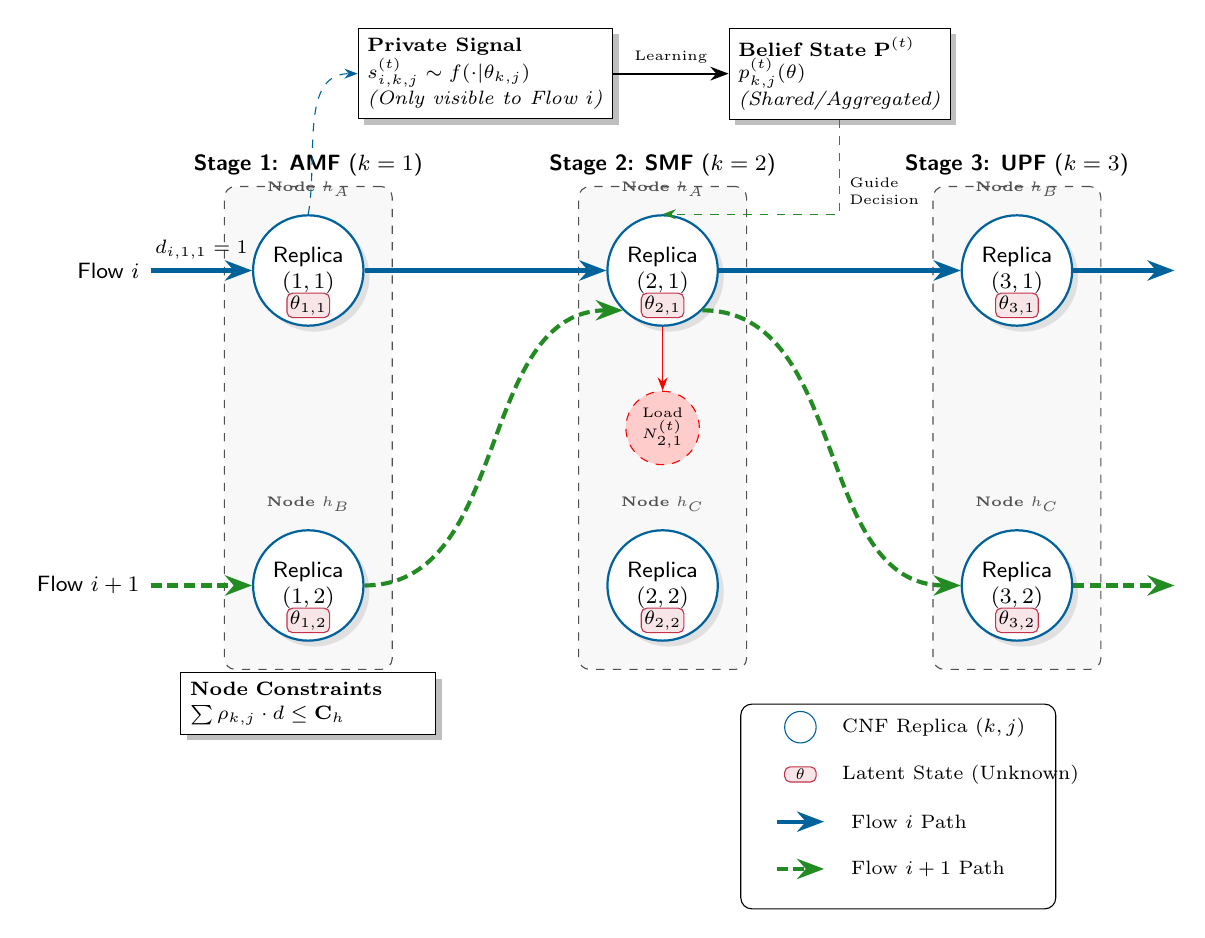
\begin{tikzpicture}[
    % Global Styles
    font=\footnotesize\sffamily,
    >=Stealth,
    % Replica Style (CNF Pod)
    replica/.style={
        circle,
        draw=ieee_blue,
        thick,
        fill=white,
        minimum size=1.4cm,
        align=center,
        drop shadow={opacity=0.2}
    },
    % Latent State Box (Inside Replica)
    latent/.style={
        rectangle,
        draw=ieee_red!80,
        fill=ieee_red!10,
        rounded corners=2pt,
        inner sep=1pt,
        font=\scriptsize
    },
    % Stage Container
    stagebox/.style={
        draw=dark_gray,
        dashed,
        rounded corners,
        fill=soft_gray!50,
        inner sep=10pt
    },
    % Flow Lines
    flow1/.style={
        ->,
        draw=ieee_blue,
        line width=1.5pt,
        rounded corners=10pt
    },
    flow2/.style={
        ->,
        draw=forest_green,
        line width=1.5pt,
        dash pattern=on 4pt off 2pt,
        rounded corners=10pt
    },
    % Annotation Box
    annot/.style={
        rectangle,
        draw=black,
        fill=white,
        drop shadow,
        font=\scriptsize,
        align=left
    }
]

% --- GRID SETUP ---
\coordinate (s1) at (0,0);
\coordinate (s2) at (4.5,0);
\coordinate (s3) at (9,0);

% --- STAGE 1: AMF ---
\node[replica] (r11) at (0, 2) {Replica\\$(1,1)$};
\node[latent, below=8pt of r11.center] (theta11) {$\theta_{1,1}$};
\node[above=0.1cm of r11, font=\tiny\bfseries, color=dark_gray] {Node $h_A$};

\node[replica] (r12) at (0, -2) {Replica\\$(1,2)$};
\node[latent, below=8pt of r12.center] (theta12) {$\theta_{1,2}$};
\node[above=0.1cm of r12, font=\tiny\bfseries, color=dark_gray] {Node $h_B$};

% --- STAGE 2: SMF ---
\node[replica] (r21) at (4.5, 2) {Replica\\$(2,1)$};
\node[latent, below=8pt of r21.center] (theta21) {$\theta_{2,1}$};
\node[above=0.1cm of r21, font=\tiny\bfseries, color=dark_gray] {Node $h_A$};

\node[replica] (r22) at (4.5, -2) {Replica\\$(2,2)$};
\node[latent, below=8pt of r22.center] (theta22) {$\theta_{2,2}$};
\node[above=0.1cm of r22, font=\tiny\bfseries, color=dark_gray] {Node $h_C$};

% --- STAGE 3: UPF ---
\node[replica] (r31) at (9, 2) {Replica\\$(3,1)$};
\node[latent, below=8pt of r31.center] (theta31) {$\theta_{3,1}$};
\node[above=0.1cm of r31, font=\tiny\bfseries, color=dark_gray] {Node $h_B$};

\node[replica] (r32) at (9, -2) {Replica\\$(3,2)$};
\node[latent, below=8pt of r32.center] (theta32) {$\theta_{3,2}$};
\node[above=0.1cm of r32, font=\tiny\bfseries, color=dark_gray] {Node $h_C$};

% --- STAGE BOUNDARIES ---
\begin{pgfonlayer}{background}
    \node[stagebox, fit=(r11) (r12), label={above:\textbf{Stage 1: AMF} ($k=1$)}] (box1) {};
    \node[stagebox, fit=(r21) (r22), label={above:\textbf{Stage 2: SMF} ($k=2$)}] (box2) {};
    \node[stagebox, fit=(r31) (r32), label={above:\textbf{Stage 3: UPF} ($k=3$)}] (box3) {};
\end{pgfonlayer}

% --- FLOWS ---

% Flow i (Blue Solid)
\coordinate (ingress1) at (-2, 2);
\coordinate (egress1) at (11, 2);
\draw[flow1] (ingress1) node[left, black] {Flow $i$} 
    -- (r11.west) 
    node[midway, above, font=\scriptsize] {$d_{i,1,1}=1$};
    
\draw[flow1] (r11.east) -- (r21.west);
\draw[flow1] (r21.east) -- (r31.west);
\draw[flow1] (r31.east) -- (egress1);

% Flow i+1 (Green Dashed) - Shows externality
\coordinate (ingress2) at (-2, -2);
\coordinate (egress2) at (11, -2);
\draw[flow2] (ingress2) node[left, black] {Flow $i+1$} 
    -- (r12.west);

% Logic: Flow i+1 chooses r12, then r21 (creating contention with flow i), then r32
\draw[flow2] (r12.east) to[out=0, in=180] (r21.south west);
\draw[flow2] (r21.south east) to[out=0, in=180] (r32.west);
\draw[flow2] (r32.east) -- (egress2);

% --- IBG ANNOTATIONS ---

% 1. Asymmetric Observation
\node (signal) at (2.25, 4.5) [annot, align=left] {
    \textbf{Private Signal}\\
    $s_{i,k,j}^{(t)} \sim f(\cdot|\theta_{k,j})$\\
    \textit{(Only visible to Flow $i$)}
};
% FIXED ARROW PATH
\draw[->, dashed, ieee_blue] (r11.north) to[out=80, in=180] (signal.west); 

% 2. Belief Update & Aggregation
\node (belief) at (6.75, 4.5) [annot, align=left] {
    \textbf{Belief State} $\mathbf{P}^{(t)}$\\
    $p_{k,j}^{(t)}(\theta)$\\
    \textit{(Shared/Aggregated)}
};
\draw[->, thick] (signal.east) -- node[above, font=\tiny] {Learning} (belief.west);

% FIXED ARROW PATH
\draw[->, dashed, forest_green] (belief.south) 
    -- (belief.south|-r21.north) coordinate (h_segment_mid) 
    -- (r21.north);
\node[above right, font=\tiny, align=left] at (h_segment_mid) {Guide\\Decision}; % Label repositioned

% 3. Negative Externality (Congestion)
\node (externality) at (4.5, 0) [circle, fill=red!20, draw=red, dashed, inner sep=2pt, align=center, font=\tiny] {Load\\$N_{2,1}^{(t)}$};
\draw[->, red] (r21.south) -- (externality.north);

% 4. Host Capacity Constraints (ADJUSTED LINE SPACING)
\node at (0, -3.5) [annot, text width=3cm] {
    \textbf{Node Constraints}\\[0.1em] % Increased space slightly
    $\sum \rho_{k,j} \cdot d \le \mathbf{C}_h$ % Removed $$ for inline-like rendering
};

% --- LEGEND (Manual Placement - ADJUSTED PLACEMENT AND SIZE) ---
\begin{scope}[shift={(8, -3.5)}, font=\scriptsize] % Shifted X coordinate to the right (from 9.5 to 10)
    % Box outline - Adjusted minimum width and added minimum height
    \node[draw, fill=white, rounded corners, inner sep=5pt, 
          minimum width=4.0cm, minimum height=2.6cm, % Increased dimensions slightly for better fit
          anchor=north east] (legend_box) at (1.5, 0) {};

    % Items (x-pos centered in box, y-pos manually spaced)
    \coordinate (start) at (-1.75, -0.3); % Start point for legend icons

    % 1. CNF Replica
    \node[circle, draw=ieee_blue, fill=white, minimum size=0.4cm] (l1_icon) at (start) {};
    \node[anchor=west] at (l1_icon.east) [xshift=2mm] {CNF Replica $(k,j)$};

    % 2. Latent State
    \node[latent, inner sep=1pt, scale=0.8, minimum width=0.5cm] (l2_icon) at ($(start) + (0, -0.6)$) {$\theta$};
    \node[anchor=west] at (l2_icon.east) [xshift=2mm] {Latent State (Unknown)};

    % 3. Flow i Path
    \draw[flow1, line width=1.5pt] ($(start) + (-0.3, -1.2)$) -- ($(start) + (0.3, -1.2)$) node[anchor=west] at ($(start) + (0.3, -1.2)$) [xshift=2mm] {Flow $i$ Path};

    % 4. Flow i+1 Path
    \draw[flow2, line width=1.5pt] ($(start) + (-0.3, -1.8)$) -- ($(start) + (0.3, -1.8)$) node[anchor=west] at ($(start) + (0.3, -1.8)$) [xshift=2mm] {Flow $i+1$ Path};
    
\end{scope}

\end{tikzpicture}
} % End \resizebox
\caption{System model of a containerized 6G core: tenant flows sequentially select CNF replicas for each SFC stage hosted across Kubernetes nodes.}
\label{fig:system_model}
\end{figure*}

This model captures the essential primitives of a distributed, containerized core: resource‑constrained hosts, heterogeneous CNFs, sequential flow arrivals, and visibility limited to per‑slot decisions.

\subsection{Performance and Uncertainty Model}
\label{sec:sys_performance}

Each CNF replica $(k,j)$ possesses an unobservable \emph{latent state} $\theta_{k,j} \in \Theta$, where $\Theta$ is a finite set of possible states representing underlying performance conditions such as host load levels or data-plane acceleration status. The true state $\theta_{k,j}$ governs the stochastic behavior of the replica's performance during a decision epoch (slot). When flow $i$ traverses replica $(k,j)$ in slot $t$, it observes a signal $s_{i,k,j}^{(t)} \in \mathcal{S}$ drawn from the conditional distribution
\begin{equation}
s_{i,k,j}^{(t)} \sim f_{k,j}(\cdot \mid \theta_{k,j}),
\label{eq:signal_model}
\end{equation}
where $f_{k,j}(\cdot \mid \theta)$ is the likelihood function specific to replica $(k,j)$ and its implementation (e.g., DPDK-accelerated vs. kernel path). Signals may represent instantaneous metrics such as processing delay, packet loss rate, or queue occupancy.

Crucially, observations are \emph{asymmetric}: only flows that select replica $(k,j)$ in slot $t$ receive direct signals about its performance. Let $\mathcal{N}_{k,j}^{(t)} = \{i : d_{i,k,j}^{(t)} = 1\}$ denote the set of flows using replica $(k,j)$ in slot $t$. These samplers observe independent signals $s_{i,k,j}^{(t)} \sim f_{k,j}(\cdot \mid \theta_{k,j})$, while non-sampling flows have no direct information about $\theta_{k,j}$. This asymmetry reflects practical constraints in multi-tenant environments where raw telemetry sharing is restricted for privacy and scalability reasons.

To manage uncertainty, each flow maintains a \emph{belief vector} $p_{k,j}^{(t)}(\theta)$ representing the estimated probability distribution over latent states $\theta \in \Theta$ for replica $(k,j)$ at the start of slot $t$. These beliefs are updated across slots using a non-Bayesian social learning rule that aggregates local observations into a shared estimate. Specifically, when flow $i$ samples replica $(k,j)$ in slot $t$, it computes a local Bayesian posterior
\begin{equation}
\mu_{i,k,j}^{(t)}(\theta) = \frac{f_{k,j}(s_{i,k,j}^{(t)} \mid \theta) p_{k,j}^{(t)}(\theta)}{\sum_{\theta' \in \Theta} f_{k,j}(s_{i,k,j}^{(t)} \mid \theta') p_{k,j}^{(t)}(\theta')},
\label{eq:local_posterior}
\end{equation}
which is then combined with others' beliefs through lightweight aggregation. Flows that do not sample the replica retain their prior belief $p_{k,j}^{(t)}(\theta)$.

The slot-based stationarity assumption holds throughout: the latent state $\theta_{k,j}$ remains fixed during slot $t$, ensuring signals collected within a slot are conditionally independent draws from $f_{k,j}(\cdot \mid \theta_{k,j})$. This enables meaningful learning from limited per-slot observations while accommodating temporal dynamics across slots. The predictive marginal distribution
\begin{equation}
\lambda_{k,j}^{(t)}(s) = \sum_{\theta \in \Theta} f_{k,j}(s \mid \theta) p_{k,j}^{(t)}(\theta),
\label{eq:predictive_marginal}
\end{equation}
serves as the sufficient statistic for expected utility calculations in subsequent decision phases.

\begin{figure*}[!t]
  \centering
  \resizebox{\textwidth}{!}{
  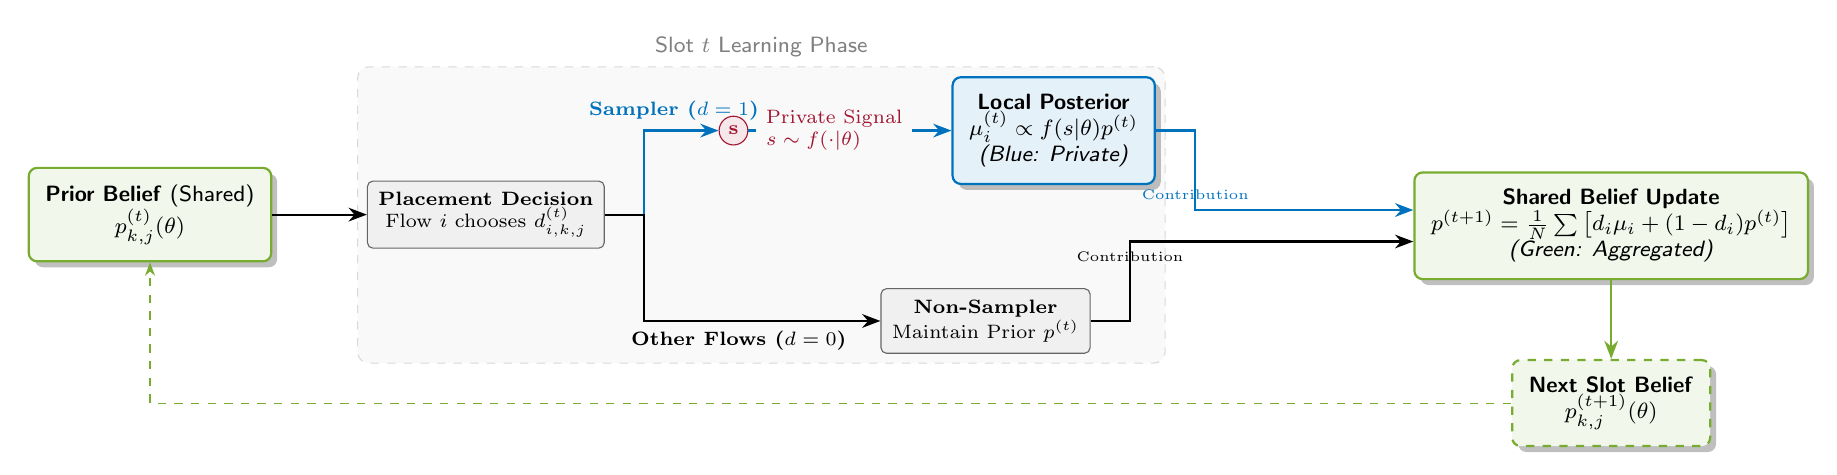
\begin{tikzpicture}[
    font=\footnotesize\sffamily,
    >=Stealth,
    node distance=1.0cm and 1.5cm,
    % Styles
    box_base/.style={
        rectangle, thick, rounded corners=3pt, align=center, drop shadow, inner sep=6pt, minimum height=1cm
    },
    shared_state/.style={
        box_base, draw=shared_green, fill=shared_green!10, text=black
    },
    local_process/.style={
        box_base, draw=local_blue, fill=local_blue!10, text=black
    },
    action_node/.style={
        rectangle, draw=black!60, fill=process_gray, rounded corners=2pt, font=\scriptsize, align=center, inner sep=4pt
    },
    signal_node/.style={
        circle, draw=signal_red, fill=signal_red!10, text=signal_red, font=\bfseries\scriptsize, inner sep=2pt
    }
]

% 1. START: Prior Belief (Shared)
\node[shared_state] (prior) {
    \textbf{Prior Belief} (Shared)\\
    $p_{k,j}^{(t)}(\theta)$
};

% 2. Decision
\node[action_node, right=1.2cm of prior] (decision) {
    \textbf{Placement Decision}\\
    Flow $i$ chooses $d_{i,k,j}^{(t)}$
};

% 3. SPLIT BRANCHES
% Top: Sampler (d=1)
\node[signal_node, above right=0.5cm and 1.5cm of decision] (signal) {s};
\node[right=0.1cm of signal, text=signal_red, font=\scriptsize, align=left] (sig_lbl) {Private Signal\\$s \sim f(\cdot|\theta)$};

\node[local_process, right=0.5cm of sig_lbl] (posterior) {
    \textbf{Local Posterior}\\
    $\mu_{i}^{(t)} \propto f(s|\theta)p^{(t)}$\\
    \textit{(Blue: Private)}
};

% Bottom: Non-Sampler (d=0)
\node[action_node, below right=0.5cm and 3.5cm of decision] (retain) {
    \textbf{Non-Sampler}\\
    Maintain Prior $p^{(t)}$
};

% 4. AGGREGATION (Green)
\node[shared_state, right=1.5cm of posterior] (aggregate) at ($(posterior)!0.5!(retain) + (3.5,0)$) {
    \textbf{Shared Belief Update}\\
    $p^{(t+1)} = \frac{1}{N} \sum \left[ d_i \mu_i + (1-d_i)p^{(t)} \right]$\\
    \textit{(Green: Aggregated)}
};

% 5. NEXT SLOT
\node[shared_state, below=1.0cm of aggregate, dashed] (next) {
    \textbf{Next Slot Belief}\\
    $p_{k,j}^{(t+1)}(\theta)$
};

% --- Connections ---
\draw[->, thick] (prior) -- (decision);

% Sampler Path (Blue)
\draw[->, thick, local_blue] (decision.east) -- ++(0.5,0) |- node[pos=0.7, above, font=\scriptsize\bfseries] {Sampler ($d=1$)} (signal.west);
\draw[->, thick, local_blue] (signal) -- (sig_lbl) -- (posterior);
\draw[->, thick, local_blue] (posterior.east) -- ++(0.5,0) |- ([yshift=0.2cm]aggregate.west) node[pos=0.5, above, font=\tiny] {Contribution};

% Non-Sampler Path (Standard)
\draw[->, thick] (decision.east) -- ++(0.5,0) |- node[pos=0.7, below, font=\scriptsize\bfseries] {Other Flows ($d=0$)} (retain.west);
\draw[->, thick] (retain.east) -- ++(0.5,0) |- ([yshift=-0.2cm]aggregate.west) node[pos=0.5, below, font=\tiny] {Contribution};

% Aggregate to Next (Green)
\draw[->, thick, shared_green] (aggregate) -- (next);
\draw[->, dashed, shared_green] (next.west) -| (prior.south);

% Background Box
\begin{scope}[on background layer]
    \node[fit=(decision)(posterior)(retain)(sig_lbl), draw=gray!30, dashed, rounded corners, fill=gray!5, label={[gray]north:Slot $t$ Learning Phase}] {};
\end{scope}

\end{tikzpicture}
} %end resize
  \caption{Non-Bayesian learning workflow: samplers compute local posteriors (blue) which are aggregated into shared beliefs (green) for future placement decisions.}
  \label{fig:learning_process}
\end{figure*}

This model captures the essential uncertainty characteristics of CNF-based 6G cores: replica performance depends on latent host conditions, observations are sparse and asymmetric, and beliefs evolve over time through collaborative inference without requiring raw telemetry exchange.


\subsection{Utility Model and Negative Externality}
\label{sec:sys_utility}

The utility of flow $i$ depends on both the intrinsic quality of selected replicas and the congestion they experience due to resource contention. For replica $(k,j)$ with latent state $\theta_{k,j}$, let $q_{i,k,j}^{(t)}$ represent the observed quality metric (e.g., processing delay or throughput) when flow $i$ traverses it in slot $t$. The per-stage utility kernel $u_k(q,n)$ is defined such that:

\begin{enumerate}
    \item $u_k(\cdot,n)$ is non-decreasing in $q$: higher observed quality yields greater utility.
    \item $u_k(q,\cdot)$ is non-increasing in $n$: more concurrent flows on the same replica degrade individual utility due to negative network externality.
\end{enumerate}

This structure captures the fundamental trade-off in SFC placement: selecting high-quality replicas improves utility, but overloading them diminishes returns. Typical instantiations include $u_k(q,n) = \alpha_k \cdot q / n$ for delay-sensitive services or $u_k(q,n) = \beta_k \cdot \log(1 + q/n)$ for throughput-oriented applications, where $\alpha_k,\beta_k>0$ are stage-specific weighting factors.

Given belief $p_{k,j}^{(t)}(\theta)$ at the start of slot $t$, the expected utility for flow $i$ selecting replica $(k,j)$ with final load $N_{k,j}^{(t)}$ is
\begin{equation}
U_{i,k}^{(t)}(j \mid N_{k,j}^{(t)}) = \sum_{\theta \in \Theta} p_{k,j}^{(t)}(\theta) \int_{\mathcal{S}} u_k(q, N_{k,j}^{(t)}) f_{k,j}(dq \mid \theta).
\label{eq:stage_expected_utility}
\end{equation}
This expression incorporates both uncertainty about replica performance (through the belief-weighted integral) and congestion effects (through $N_{k,j}^{(t)}$).

The end-to-end utility combines per-stage contributions with deterministic link costs between consecutive stages:
\begin{equation}
U_i^{(t)} = \sum_{k=1}^{K} U_{i,k}^{(t)}(d_{i,k}^{(t)} \mid N_{k,d_{i,k}^{(t)}}^{(t)}) - \sum_{k=1}^{K-1} L_{\text{link}}(h(d_{i,k}^{(t)}), h(d_{i,k+1}^{(t)})),
\label{eq:e2e_utility}
\end{equation}
where $L_{\text{link}}(h,h')$ denotes the latency or cost of communication between nodes hosting consecutive replicas. The additive composition assumes no cross-stage coupling beyond link costs—a reasonable approximation when stages operate independently (e.g., stateless microservices).

Figure~\ref{fig:utility_function} illustrates how the utility kernel $u_k(q,n)$ decreases with increasing load $n$ for fixed quality $q$, demonstrating the negative externality effect. This congestion-sensitive utility model ensures that flows anticipate reduced performance when many others select the same replica, leading to strategic diversification in placement decisions.

\begin{figure}[!t]
  \centering
  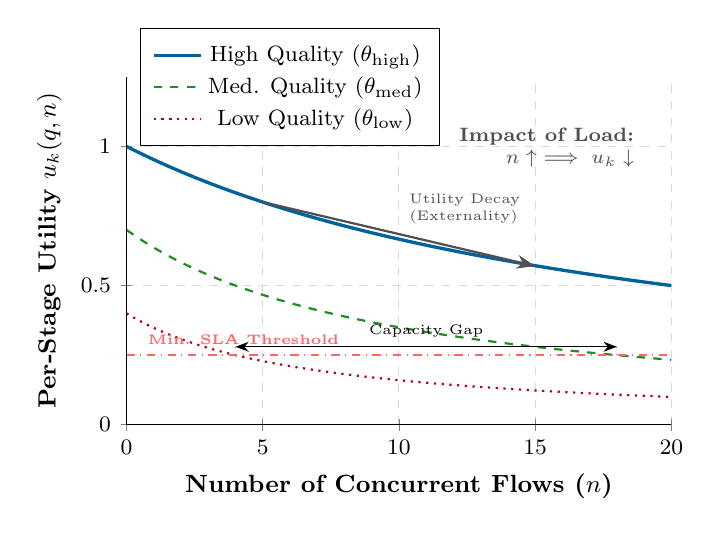
\begin{tikzpicture}
\begin{axis}[
    % Axis Setup
    width=8.5cm, height=6cm,
    xlabel={Number of Concurrent Flows ($n$)},
    ylabel={Per-Stage Utility $u_k(q,n)$},
    xmin=0, xmax=20,
    ymin=0, 
    ymax=1.25, % Retain max y-axis for spacing
    axis lines=left,
    grid=major,
    grid style={dashed, gray!30},
    ylabel style={font=\small\bfseries, align=center},
    xlabel style={font=\small\bfseries},
    tick label style={font=\footnotesize},
    % Legend Style (Moved slightly lower)
    legend style={
        at={(0.3, 0.8)}, 
        anchor=south,
        font=\footnotesize, 
        fill=white, 
        draw=black, 
        fill opacity=1.0,
        inner sep=4pt,
        nodes={inner sep=2pt}
    },
    % Clean look
    axis line style={-},
    clip mode=individual 
]

    % --- PLOTS ---
    % Model: U = q / (1 + beta * n)

    % 1. High Quality Replica (theta_high)
    \addplot[
        color=ieee_blue,
        very thick,
        domain=0:20,
        samples=100,
        smooth
    ]
    {1.0 / (1 + 0.05*x)};
    \addlegendentry{High Quality ($\theta_{\text{high}}$)}

    % 2. Medium Quality Replica (theta_med)
    \addplot[
        color=forest_green,
        thick,
        dashed,
        domain=0:20,
        samples=100,
        smooth
    ]
    {0.7 / (1 + 0.1*x)};
    \addlegendentry{Med. Quality ($\theta_{\text{med}}$)}

    % 3. Low Quality Replica (theta_low)
    \addplot[
        color=ieee_red,
        thick,
        dotted,
        domain=0:20,
        samples=100,
        smooth
    ]
    {0.4 / (1 + 0.15*x)};
    \addlegendentry{Low Quality ($\theta_{\text{low}}$)}

    % --- ANNOTATIONS ---
    
    % SLA Threshold Line
    \draw[red!60, dashdotted, line width=0.8pt] (axis cs:0,0.25) -- (axis cs:20,0.25) 
        node[pos=0.02, above right, font=\tiny\bfseries] {Min. SLA Threshold};

    % Negative Externality Arrow (Utility Decay)
    \draw[->, >=Stealth, thick, dark_gray] (axis cs: 5, 0.8) -- (axis cs: 15, 0.57) 
        node[midway, above right, font=\tiny, align=left] {Utility Decay\\(Externality)};

    % Capacity Gap Arrow
    \draw[<->, >=Stealth, thin, black] (axis cs: 4, 0.28) -- (axis cs: 18, 0.28)
        node[midway, above, font=\tiny] {Capacity Gap};
    
    % Dotted lines to show the x-values for capacity gap
    \draw[dotted, gray] (axis cs: 4, 0.25) -- (axis cs: 4, 0.28);
    \draw[dotted, gray] (axis cs: 18, 0.25) -- (axis cs: 18, 0.28);

    % General Text Label - Remains in the north east corner, now clearly visible
    \node[anchor=north east, font=\scriptsize, align=right, text=dark_gray] at (axis cs: 19, 1.1) {
        \textbf{Impact of Load:}\\
        $n \uparrow \implies u_k \downarrow$
    };

\end{axis}
\end{tikzpicture}
  \caption{Per-stage utility kernel showing negative externality: utility decreases as the number of concurrent flows ($n$) on a replica increases, even for fixed quality ($q$).}
  \label{fig:utility_function}
\end{figure}

This utility structure formalizes the core challenge: flows must balance selecting high-quality replicas against avoiding congestion, requiring both accurate belief estimation and strategic anticipation of others' decisions.


\subsection{Problem Statement}
\label{sec:sys_problem}

The overarching objective is to devise a distributed placement policy that maximizes the aggregate utility of all admitted flows over time, subject to resource constraints and informational limitations. Formally, we seek to maximize the expected social welfare, defined as the sum of all flow utilities in a given slot $t$:
\begin{equation}
\max_{\{d_{i,k,j}^{(t)}\}} \mathbb{E} \left[ \sum_{i \in \mathcal{N}} U_i^{(t)} \right],
\label{eq:social_welfare}
\end{equation}
where the expectation is taken over the stochastic signals and the randomness in flow arrivals.

This optimization is subject to the following constraints:
\begin{align}
& \sum_{j \in \mathcal{I}_k} d_{i,k,j}^{(t)} = 1, && \forall i \in \mathcal{N}, k \in \mathcal{T} \quad \text{(One replica per stage)} \label{eq:constraint_one_per_stage} \\
& \sum_{i \in \mathcal{N}} d_{i,k,j}^{(t)} \cdot \boldsymbol{\rho}_{k,j} \le \mathbf{C}_{h(k,j)}, && \forall (k,j) \in \mathcal{I} \quad \text{(Node capacity)} \label{eq:constraint_node_cap} \\
& d_{i,k,j}^{(t)} \in \{0,1\}, && \forall i,k,j \quad \text{(Binary placement)} \label{eq:constraint_binary} \\
& d_{i,k,j}^{(t)} \le a_{k,j}^{(t)}, && \forall i,k,j \quad \text{(Replica availability)} \label{eq:constraint_availability}
\end{align}

Solving this problem is exceptionally challenging due to three intertwined factors. First, the **strategic interdependence** of decisions means that the utility of any flow $i$ depends not only on its own choices but also on the concurrent choices of all other flows through the load terms $N_{k,j}^{(t)}$. Second, the **sequential nature** of arrivals implies that early decisions create externalities that directly impact the utility of later flows, requiring forward-looking strategies. Third, the **incomplete information**—where replica states $\theta_{k,j}$ are latent and only partially observed—means that decisions must be made under uncertainty.

A myopic solution that optimizes for immediate utility without considering future impacts is suboptimal. Likewise, a centralized solution is infeasible due to scalability and privacy constraints. Therefore, the problem is best formulated as a sequential game of incomplete information, where the goal is to find a solution concept that is both stable and individually rational. We seek a placement strategy profile that constitutes a **Subgame-Perfect Nash Equilibrium (SPNE)**. An SPNE is a set of strategies where, at every decision point in the game (for every flow $i$, given the actions of all preceding flows), no player can unilaterally deviate and improve its expected utility, given its beliefs about the system state.

Formally, the problem is to find a strategy profile $\mathbf{d}^* = \{d_1^*, \dots, d_N^*\}$ such that for every flow $i \in \mathcal{N}$, every possible history of play $\mathcal{H}_{i-1}$, and every feasible alternative action $d_i' \neq d_i^*$, the following holds:
\begin{equation}
U_i^{(t)}(d_i^* \mid \mathcal{H}_{i-1}, \mathbf{p}^{(t)}) \ge U_i^{(t)}(d_i' \mid \mathcal{H}_{i-1}, \mathbf{p}^{(t)}),
\label{eq:spne_condition}
\end{equation}
where $\mathbf{p}^{(t)}$ represents the vector of beliefs for all replicas at the start of the slot.

The subsequent sections of this paper are dedicated to constructing such an equilibrium using the Indian Buffet Game framework, developing algorithms to compute it, and proving its properties.


\section{The Indian Buffet Game Framework for SFC}
\label{sec:ibg_framework}

\subsection{The IBG Analogy: Mapping SFC to Dishes and Customers}
\label{sec:ibg_analogy}

We model distributed SFC placement as an \emph{Indian Buffet Game} (IBG), a strategic sequential game in which rational players select from a set of latent-quality items under uncertainty and negative externality. The analogy between SFC placement and an Indian buffet is direct and functionally precise:

\begin{itemize}
    \item \textbf{Flows} $\leftrightarrow$ \textbf{Customers}: Each tenant flow $i$ arriving in a decision slot corresponds to a customer entering the buffet sequentially.
    \item \textbf{CNF Replicas} $\leftrightarrow$ \textbf{Dishes}: Each CNF replica $(k,j)$ at stage $k$ is a dish $r_{k,j}$, with unknown but time-invariant latent quality $\theta_{k,j}$.
    \item \textbf{SFC Stage} $\leftrightarrow$ \textbf{Buffet Station}: Each SFC stage $k$ is a distinct buffet station offering $M_k$ dishes (replicas); a flow must select one dish per station to complete its meal (service chain).
    \item \textbf{Latent State} $\leftrightarrow$ \textbf{Dish Quality}: The unobserved performance state $\theta_{k,j}$ determines the statistical distribution of signal quality $s_{i,k,j}^{(t)}$ (e.g., processing delay), analogous to how a dish’s true deliciousness governs its taste.
    \item \textbf{Signal Observation} $\leftrightarrow$ \textbf{Tasting}: Only customers who select a dish observe its true quality via a noisy signal $s_{i,k,j}^{(t)}$; others remain uncertain, relying on others’ choices and aggregated summaries.
    \item \textbf{Negative Externality} $\leftrightarrow$ \textbf{Congestion}: As more customers select the same dish, the utility per customer decreases due to overcrowding or diminished portion size—mirroring how increased load on a CNF replica degrades per-flow latency or throughput.
\end{itemize}

This analogy is not merely illustrative—it captures the core structural properties of the SFC placement problem: sequential decision-making, incomplete information, asymmetric observations, and congestion-driven utility degradation. The IBG framework thus provides a natural, rigorous mathematical structure to model how flows learn replica performance from limited, private signals and make strategic placement decisions that account for the impact of prior and future choices.

The key innovation lies in extending the non-strategic Indian Buffet Process—used in machine learning for non-parametric Bayesian modeling—to a \emph{strategic} setting where agents actively learn, predict, and optimize under uncertainty. This enables the design of distributed, equilibrium-based placement algorithms that are both theoretically grounded and practically implementable in 6G core networks.

\begin{table}[!t]
\centering
\caption{Mapping between SFC Placement and the Indian Buffet Game}
\label{tab:ibg_mapping}
\begin{tabular}{ll}
\toprule
\textbf{SFC Placement} & \textbf{Indian Buffet Game} \\
\midrule
Tenant flow $i$ & Customer $i$ \\
CNF replica $(k,j)$ & Dish $r_{k,j}$ \\
SFC stage $k$ & Buffet station $k$ \\
Latent state $\theta_{k,j}$ & True dish quality \\
Observed signal $s_{i,k,j}^{(t)}$ & Taste experience \\
Belief $p_{k,j}^{(t)}(\theta)$ & Estimated dish quality distribution \\
Pre-decision count $n_{k,j}^{(t)}(m-1)$ & Number of prior customers at dish $r_{k,j}$ \\
Final load $N_{k,j}^{(t)}$ & Total customers at dish $r_{k,j}$ \\
Utility $u_k(q,n)$ & Satisfaction from dish quality and crowding \\
Control-plane belief exchange & Sharing taste impressions among diners \\
\bottomrule
\end{tabular}
\end{table}

Table~\ref{tab:ibg_mapping} summarizes this one-to-one mapping, providing a concise reference for the formal game-theoretic formulation in the following subsection.


\subsection{Formal Game-Theoretic Model}
\label{sec:ibg_formal_model}

We define the Indian Buffet Game for SFC placement at slot $t$ as a finite, sequential-move game with imperfect information, denoted by $\mathcal{G}^{(t)} = (\mathcal{N}, \mathcal{R}, \mathcal{X}, U(\cdot; \mathbf{P}^{(t)}))$, where:

\begin{itemize}
    \item $\mathcal{N} = \{1,\dots,N\}$ is the set of players (tenant flows),
    \item $\mathcal{R} = \bigcup_{k=1}^K \{(k,j) : j \in \mathcal{I}_k\}$ is the set of available dishes (active CNF replicas),
    \item $\mathcal{X} = \prod_{i=1}^N \mathcal{X}_i$ is the joint strategy space, where each player $i$ selects a strategy $\mathbf{d}_i = (d_{i,1}, \dots, d_{i,K})$ with $d_{i,k} \in \mathcal{I}_k$ indicating the chosen replica at stage $k$, subject to feasibility constraints (Eq.~\eqref{eq:one_per_stage} and availability),
    \item $U(\cdot; \mathbf{P}^{(t)}) = (U_1^{(t)}, \dots, U_N^{(t)})$ is the vector of expected utility functions parameterized by the belief profile $\mathbf{P}^{(t)} = \{p_{k,j}^{(t)}(\theta)\}_{(k,j)\in\mathcal{R}}$, where $U_i^{(t)}$ is given by Eq.~\eqref{eq:e2e_utility}.
\end{itemize}

The game proceeds in a fixed decision order $\pi^{(t)}$, where player $\pi^{(t)}(1)$ moves first, followed by $\pi^{(t)}(2)$, and so on. Each player $i = \pi^{(t)}(m)$ observes the actions of all previous players through the pre-decision counts $n_{k,j}^{(t)}(m-1)$, but does not observe the private signals $s_{i',k,j}^{(t)}$ collected by earlier samplers unless aggregated into the belief $\mathbf{P}^{(t)}$. The game ends after all $N$ players have chosen their SFC paths, yielding a strategy profile $\mathbf{D}^{(t)} = (\mathbf{d}_1^{(t)}, \dots, \mathbf{d}_N^{(t)})$ and resulting in the final replica loads $N_{k,j}^{(t)}$.

A pure-strategy profile $\mathbf{D}^*$ is a \emph{Subgame-Perfect Nash Equilibrium} (SPNE) if, for every subgame starting at any decision position $m$ and given belief $\mathbf{P}^{(t)}$, the action $\mathbf{d}_{\pi^{(t)}(m)}^*$ is a best response to the continuation strategies of players $\pi^{(t)}(m+1), \dots, \pi^{(t)}(N)$.

This formulation captures the essence of strategic SFC placement: each flow must anticipate how its choice affects not only its own utility but also the incentives of later flows, all while learning the true performance of replicas from partial observations.

\subsection{Information Structure and Subgames}
\label{sec:ibg_subgames}

The game $\mathcal{G}^{(t)}$ features a hierarchical information structure. At the time of its decision, player $i = \pi^{(t)}(m)$ observes the history $H_m = \{ n_{k,j}^{(t)}(m-1) \}_{(k,j)\in\mathcal{R}}$—the number of prior selections per replica—but not the private signals $s_{i',k,j}^{(t)}$ of earlier samplers. However, all players share a common belief $\mathbf{P}^{(t)}$ about replica states, updated from prior slots via non-Bayesian aggregation (Eq.~\eqref{eq:nonbayes_update_repeat}). This belief serves as the only mechanism for information sharing across non-sampling players.

A \emph{subgame} $\mathcal{G}^{(t)}_m$ is defined by the triplet $(m, H_m, \mathbf{P}^{(t)})$, representing the game starting at decision position $m$, given the observed pre-decision counts and the current belief profile. The subgame includes all remaining players $\{\pi^{(t)}(m), \dots, \pi^{(t)}(N)\}$ and their feasible strategies under the constraints of $H_m$ and $\mathbf{P}^{(t)}$.

The SPNE is defined recursively: for the terminal subgame ($m=N$), player $N$ selects a best response using the current belief and observed counts. For earlier subgames, each player $m$ computes a best response assuming that all subsequent players will play according to their own SPNE strategies in their respective subgames. This backward-induction structure ensures that equilibrium strategies are optimal not only at the root but in every subgame, eliminating non-credible threats and ensuring dynamic consistency.

This information structure is critical: it reflects real-world deployment constraints where raw telemetry is never shared, but aggregated beliefs (e.g., compressed posterior vectors or sufficient statistics) are exchanged via lightweight control-plane messages (e.g., NSM/NSE sidecars). The SPNE under this asymmetric information regime ensures that placement decisions are both strategically rational and privacy-aware, forming the foundation for the exact and approximate algorithms presented in Sections~\ref{sec:exact_algorithms} and~\ref{sec:approximations}.

\section{Equilibrium Computation: Exact Algorithms}
\label{sec:algorithms_exact}

This section presents recursive algorithms to compute Subgame-Perfect Nash Equilibria (SPNE) for the Indian Buffet Game formulation. We first address the computationally tractable decoupled case, where the problem decomposes into independent per-stage games. This provides a foundation and a benchmark for the more complex, NP-hard budgeted case addressed in Section V.B.

\subsection{The Decoupled Case: Per-Stage Elementary IBG}
\label{sec:exact_decoupled}

When the end-to-end utility is additive across stages — as assumed in Eq.~\eqref{eq:e2e_utility} — the SFC placement problem decomposes into $K$ independent elementary Indian Buffet Games (IBGs), one for each stage $k \in \mathcal{T}$. In this regime, the utility of a flow’s choice at stage $k$ depends only on the load at that stage and the belief about its replicas, and is unaffected by selections at other stages (beyond fixed link costs). This decoupling enables each stage to be solved independently, without global coordination or joint optimization.

The algorithm, \textsf{BR\_EIBG} (Algorithm~\ref{alg:br_eibg}), implements backward induction. It computes the optimal action for each player (flow) by anticipating the optimal actions of all subsequent players. The key to its efficiency is memoization: the results of subproblems are cached to avoid re-computation. A subproblem is defined by the tuple $(i, n_i)$, where $i$ is the current player's turn and $n_i$ is the number of players who have already chosen the replica. Since $n_i \in \{0, \dots, N-1\}$, the total number of unique states is bounded by $O(N^2)$, making the algorithm polynomial in the number of flows.

\begin{algorithm}[!t]
\caption{\textsf{BR\_EIBG}$(p_{k,\cdot}, n_i, i)$ — Backward induction for the elementary IBG}
\label{alg:br_eibg}
\DontPrintSemicolon
\KwIn{Belief vector $p_{k,j}=\{p_{k,j}(\theta)\}_{j,\theta}$; pre-decision count $n_i$; player index $i\in\{1,\dots,N\}$.}
\KwOut{Tuple $(d_i^\star, m_i)$ where $d_i^\star\in\{0,1\}$ is the optimal action and $m_i$ is the predicted number of later choosers.}
\BlankLine
\SetKwFunction{EvalUtil}{EvalUtil}
\Fn{\EvalUtil{$n$}}{
  \tcp{Expected stage utility with total sharers $n$}
  \Return $\displaystyle \sum_{\theta\in\Theta} p_{k,j}(\theta)\; \int_{\mathcal S} u_k(q,n)\,f_{k,j}(dq\mid \theta)$\;
}
\BlankLine
\If{$i==N$}{
  \tcp{Last player: evaluate directly}
  $U \leftarrow$ \EvalUtil{$n_i+1$}\;
  \uIf{$U>0$}{$d_i^\star \leftarrow 1$}
  \Else{$d_i^\star \leftarrow 0$}
  $m_i \leftarrow 0$\;
  \Return $(d_i^\star, m_i)$\;
}
\Else{
  \tcp{Branch A: assume player $i$ chooses}
  $(d_{i+1}^{(1)},m_{i+1}^{(1)}) \leftarrow \textsf{BR\_EIBG}(p_{k,\cdot},\,n_i+1,\,i+1)$\;
  $m^{(1)} \leftarrow m_{i+1}^{(1)} + d_{i+1}^{(1)}$\;
  $U^{(1)} \leftarrow$ \EvalUtil{$n_i+m^{(1)}+1$}\;
  \If{$U^{(1)}>0$}{
    $d_i^\star \leftarrow 1;\; m_i \leftarrow m^{(1)}$\;
    \Return $(d_i^\star, m_i)$\;
  }
  \tcp{Branch B: assume player $i$ skips}
  $(d_{i+1}^{(0)},m_{i+1}^{(0)}) \leftarrow \textsf{BR\_EIBG}(p_{k,\cdot},\,n_i,\,i+1)$\;
  $m_i \leftarrow m_{i+1}^{(0)} + d_{i+1}^{(0)}$\;
  $d_i^\star \leftarrow 0$\;
  \Return $(d_i^\star, m_i)$\;
}
\end{algorithm}

\begin{theorem}[SPNE for the Decoupled Case]
\label{thm:br_eibg_spne}
The strategy profile generated by invoking \textsf{BR\_EIBG} for each stage $k \in \mathcal{T}$ with initial counts $n_1=0$ constitutes a Subgame-Perfect Nash Equilibrium for the decoupled SFC placement problem.
\end{theorem}
\begin{proof}
The proof follows from the principle of backward induction and is detailed in Appendix A. The additive utility assumption ensures that the optimal action at stage $k$ is independent of the actions taken at other stages.
\end{proof}

The computational complexity of \textsf{BR\_EIBG} is significantly lower than its worst-case appearance suggests. With memoization, each unique state $(i, n_i)$ is evaluated only once. The number of such states is at most $N \times N = O(N^2)$. Each state evaluation involves a constant number of calls to \textsf{EvalUtil}, whose cost we denote $C_{\mathrm{eval}} = O(|\Theta| \cdot |\mathcal{S}|)$. Therefore, the total complexity per stage is $O(N^2 \cdot C_{\mathrm{eval}})$. Across all $K$ stages, the complexity is $\sum_{k=1}^K O(N^2 \cdot C_{\mathrm{eval}}^{(k)})$. In practice, many states are unreachable, often leading to a near-linear runtime of $O(N \cdot C_{\mathrm{eval}})$.

This polynomial-time solution is highly practical for the decoupled regime. However, as we will see, introducing a per-flow budget constraint transforms the problem into a computationally prohibitive one, necessitating the scalable approximations developed in Section VI.


\subsection{The Budgeted Case: Combinatorial IBG}
\label{sec:exact_budgeted}

When each flow is constrained to select at most $L < M$ replicas across all stages — due to per-flow budget limits, host capacity caps, or operational policies — the additive decomposition no longer holds. Choices at one stage now compete for shared resources with choices at other stages, creating a combinatorial coupling that renders the problem fundamentally interdependent. In this regime, a flow’s strategy is a binary vector $\mathbf{d}_i = (d_{i,1}, \dots, d_{i,M}) \in \{0,1\}^M$, where $M = \sum_{k=1}^K M_k$ is the total number of replicas, and $\sum_{j=1}^M d_{i,j} \leq L$. The feasible set of combinations is $\Phi = \left\{ \boldsymbol{\phi} \in \{0,1\}^M : 1 \leq \sum_{j=1}^M \phi_j \leq L \right\}$, with cardinality $H = \sum_{\ell=1}^L \binom{M}{\ell}$.

The expected utility for flow $i$ selecting combination $\boldsymbol{\phi}$, given pre-decision count vector $\mathbf{n}_i = (n_{i,1}, \dots, n_{i,M})$ and belief profile $\mathbf{P}^{(t)}$, is:
\begin{align}
U_i(\boldsymbol{\phi} \mid \mathbf{n}_i)
&= \sum_{j=1}^M \phi_j
   \sum_{\theta \in \Theta} p_{j}^{(t)}(\theta)
   \int_{\mathcal{S}} \!
   u_j\!\big(q,\, n_{i,j} + m_j + \phi_j\big)
   \notag\\
&\quad\times f_j(dq \mid \theta).
\label{eq:Ui_split}
\end{align}


where $m_j$ is the predicted number of subsequent players selecting replica $j$, and $n_{i,j} + m_j + \phi_j$ is the estimated total load on replica $j$. Unlike the decoupled case, the utility of selecting a replica at stage $k$ now depends on how many other replicas from *other* stages are selected by the same flow — due to shared budget constraints and potential co-location on the same host.

To compute the SPNE under this coupling, we extend backward induction to handle combinatorial actions. The algorithm $\textsf{BR\_IBG}(\mathbf{P}, \mathbf{n}_i, i)$ recursively evaluates all feasible combinations $\boldsymbol{\phi} \in \Phi$ for player $i$, simulates the continuation game under each, and selects the combination yielding maximum expected utility.

\begin{algorithm}[t]
\DontPrintSemicolon
\SetAlgoLined
\caption{$\textsf{BR\_IBG}(\mathbf{P}, \mathbf{n}_i, i)$ — Best Response for Budgeted IBG}
\label{alg:br_ibg}
\KwIn{Belief profile $\mathbf{P} = \{p_j(\theta)\}_{j=1,\dots,M,\;\theta\in\Theta}$; pre-decision count vector $\mathbf{n}_i = (n_{i,1},\dots,n_{i,M})$; player index $i \in \{1,\dots,N\}$; budget $L$}
\KwOut{Optimal combination $\mathbf{d}_i^* \in \Phi$; predicted future selections $\mathbf{m}_i$}
\BlankLine
\SetKwFunction{EvalUtilComb}{EvalUtilComb}
\Fn{\EvalUtilComb{$\mathbf{P}, \mathbf{n}, \boldsymbol{\phi}$}}{
    \Return $\displaystyle \sum_{j=1}^M \phi_j \sum_{\theta \in \Theta} p_j(\theta) \int_{\mathcal{S}} u_j(q, n_j + \phi_j) f_j(dq \mid \theta)$\;
}
\BlankLine
\uIf{$i = N$}{
    \ForEach{$\boldsymbol{\phi} \in \Phi$}{
        $U(\boldsymbol{\phi}) \leftarrow \EvalUtilComb(\mathbf{P}, \mathbf{n}_i, \boldsymbol{\phi})$\;
    }
    $\boldsymbol{\phi}^* \leftarrow \arg\max_{\boldsymbol{\phi} \in \Phi} U(\boldsymbol{\phi})$\;
    $\mathbf{d}_i^* \leftarrow \boldsymbol{\phi}^*$; $\mathbf{m}_i \leftarrow \mathbf{0}$\;
}
\Else{
    \ForEach{$\boldsymbol{\phi} \in \Phi$}{
        \tcp{Predict continuation under $\boldsymbol{\phi}$}
        $(\mathbf{d}_{i+1}, \mathbf{m}_{i+1}) \leftarrow \textsf{BR\_IBG}(\mathbf{P}, \mathbf{n}_i + \boldsymbol{\phi}, i+1)$\;
        $\mathbf{m}_i^{(\boldsymbol{\phi})} \leftarrow \mathbf{m}_{i+1} + \mathbf{d}_{i+1}$\;
        \tcp{Evaluate utility using predicted future loads}
        $U(\boldsymbol{\phi}) \leftarrow \displaystyle \sum_{j=1}^M \phi_j \sum_{\theta \in \Theta} p_j(\theta) \int_{\mathcal{S}} u_j(q, n_{i,j} + m_{i,j}^{(\boldsymbol{\phi})} + \phi_j) f_j(dq \mid \theta)$\;
    }
    $\boldsymbol{\phi}^* \leftarrow \arg\max_{\boldsymbol{\phi} \in \Phi} U(\boldsymbol{\phi})$\;
    $\mathbf{d}_i^* \leftarrow \boldsymbol{\phi}^*$; $\mathbf{m}_i \leftarrow \mathbf{m}_i^{(\boldsymbol{\phi}^*)}$\;
}
\Return $(\mathbf{d}_i^*, \mathbf{m}_i)$\;
\end{algorithm}

The algorithm exhaustively enumerates all $H$ feasible combinations for each player, recursively predicting the equilibrium behavior of subsequent players under each candidate. For each $\boldsymbol{\phi}$, it computes the predicted future load $\mathbf{m}_i^{(\boldsymbol{\phi})}$ by simulating the continuation game, then evaluates the total expected utility under that scenario. The optimal $\boldsymbol{\phi}^*$ is selected as the one maximizing this utility.

\begin{theorem}[SPNE for Budgeted Case]
\label{thm:br_ibg_spne}
Fix belief profile $\mathbf{P}$ and budget $L$. Invoking $\textsf{BR\_IBG}(\mathbf{P}, \mathbf{0}, 1)$ returns a strategy profile $\mathbf{D}^* = (\mathbf{d}_1^*, \dots, \mathbf{d}_N^*)$ that constitutes a subgame-perfect Nash equilibrium of the budgeted IBG.
\end{theorem}

\begin{proof}[Sketch]
The algorithm performs backward induction over a finite sequential game with finite action sets. At the terminal player $N$, the best response is found by exhaustive search over $\Phi$. Assuming the algorithm returns SPNE for all subgames starting at $i+1$, player $i$ selects the combination $\boldsymbol{\phi}^*$ that maximizes their expected utility given the predicted continuation play. By induction, the resulting profile is a best response in every subgame, hence an SPNE. Full proof in Appendix~B.
\end{proof}

\begin{remark}[Computational Hardness]
The per-player optimization problem embedded in $\textsf{BR\_IBG}$ — selecting up to $L$ items from $M$ to maximize a non-linear, load-dependent utility — is NP-hard, as it generalizes the cardinality-constrained knapsack problem. Consequently, the full SPNE computation is exponential in $M$ and $L$. The worst-case time complexity with memoization is $O\big(N \cdot (N+1)^M \cdot H \cdot C_{\text{eval}}\big)$, where $C_{\text{eval}}$ is the cost of evaluating one utility term. This renders the exact algorithm infeasible for $M > 20$ or $L > 5$, motivating the scalable approximations in Section~\ref{sec:approximations}.
\end{remark}

\begin{remark}[SFC-Specific Constraint]
While the general Budgeted IBG allows players to select any subset of items up to size $L$, in the specific context of SFC, the budget is fixed to the chain length ($L=K$), and the constraint becomes strict: players must select exactly one replica per stage. The computational hardness arises not from the number of items chosen, but from the combinatorial coupling of joint selections across stages (e.g., link delays and shared node capacities) which prevents independent per-stage optimization.
\end{remark}

While $\textsf{BR\_IBG}$ guarantees an SPNE, its computational burden makes it impractical for operational 6G cores. Nevertheless, it serves as a critical benchmark for validating approximate algorithms and provides theoretical grounding for the distributed, learning-driven placement framework. The next section introduces a suite of practical approximations that preserve the core strategic and learning elements while achieving near-optimal performance with low overhead.


\section{Scalable Approximations for Large-Scale Deployments}
\label{sec:approximations}

The exponential complexity of \textsf{BR\_IBG} (Section V.B) renders it computationally infeasible for real-time placement in large-scale 6G cores, where hundreds of replicas and thousands of flows must be managed per slot. To bridge this gap, we develop a suite of scalable approximation heuristics. These are not ad-hoc rules but are grounded in the same game-theoretic and learning principles, designed to deliver near-optimal performance with drastically lower computational and communication overhead.

\subsection{Design Principles for Practical Heuristics}
\label{sec:approx_principles}

Before presenting the specific algorithms, we establish the core design principles that guide their development. These principles ensure that our approximations are not only fast but also retain the strategic essence of the IBG framework.

\begin{itemize}
    \item \textbf{Tractability and Low Complexity:} Algorithms must have polynomial or near-linear complexity in the number of flows ($N$) and replicas ($M$). They should avoid combinatorial explosion at all costs.
    
    \item \textbf{Information Frugality and Low Overhead:} Heuristics should operate with limited, local information. They must not require global state visibility or extensive telemetry exchange, keeping the control-plane overhead ($B^{(t)}$) minimal.
    
    \item \textbf{Strategic Fidelity:} Crucially, they must approximate strategic reasoning. A purely myopic greedy algorithm is insufficient. Our heuristics incorporate elements of lookahead, pruning, or stochastic sampling to anticipate the actions and congestion caused by subsequent flows.
    
    \item \textbf{Robustness and Adaptability:} The heuristics must perform well under noisy beliefs and high churn (frequent replica scaling events), gracefully adapting to the dynamic 6G environment.
    
    \item \textbf{Tunability:} Provide operators with tunable knobs (e.g., candidate set size $C$, lookahead depth $D$, number of samples $S$) to balance the trade-off between solution quality and runtime/overhead for their specific deployment.
\end{itemize}

The following subsection presents a catalog of such heuristics, progressing from simple myopic rules to more sophisticated lookahead and stochastic methods, culminating in practical implementation guidance.


\subsection{A Catalog of Approximation Heuristics}
\label{sec:approx_catalog}

We now present a suite of scalable heuristics designed to approximate the SPNE solution. To address the computational intractability of the budgeted IBG, we adopt a **pipelined design philosophy**: simple heuristics (like greedy selection or pruning) serve as pre-processing steps or simulation policies for more advanced strategies (like lookahead). This composition allows us to trade optimality for polynomial-time complexity while retaining strategic foresight.

\subsubsection{Greedy Per-Stage Myopic Best-Response}
\label{sec:approx_greedy}

The simplest approximation treats each SFC stage independently and selects, for each arriving flow, the replica that maximizes the immediate expected utility under the current belief $\mathbf{P}^{(t)}$ and observed pre-decision counts. For stage $k$, flow $i$ computes $U_{i,k}(j \mid n_{i,k,j}^{(t)} + 1)$ for all feasible replicas $j \in \mathcal{I}_k$ and selects the one with the highest positive value. This approach is purely myopic, ignoring the impact of the current decision on future flows and neglecting cross-stage coupling (except for link costs). However, its low computational cost ($O(M \cdot C_{\text{eval}})$ per flow) makes it an essential building block: we utilize this greedy policy as the default "simulation policy" for the more advanced lookahead and Monte Carlo algorithms described below.

\subsubsection{Candidate Pruning with Local Search}
\label{sec:approx_pruning}

To mitigate the combinatorial explosion of the action space, we employ a pre-filtering technique. For each stage, we retain only the top $C$ candidates ranked by a static score (expected utility under zero congestion, adjusted for baseline capacity $\kappa_{k,j}$). We denote this reduced action space as $\Phi_C \subset \Phi$, where the cardinality is bounded by the pruning factor $C$ (i.e., $|\Phi_C| \approx C^K \ll M^K$). 

Once the space is pruned, the flow solves the constrained optimization over $\Phi_C$. If $C$ is small (e.g., $C \in \{5,8\}$), exhaustive enumeration is feasible. For slightly larger $C$, we apply local search (e.g., best-improvement hill-climbing) to iteratively swap replicas within the pruned set. This method drastically reduces the search space from exponential in $M$ to polynomial in $C$, creating a tractable foundation for the lookahead mechanisms.

\subsubsection{Pruned Lookahead Rollout}
\label{sec:approx_lookahead}

Pure lookahead on the full action space is intractable due to the branching factor $O(M^K)$. To capture strategic effects in large-scale topologies, we employ a \textit{staged pipeline}: we first apply the Candidate Pruning heuristic (Sec.~\ref{sec:approx_pruning}) to generate the reduced set $\Phi_C$, and then execute the lookahead mechanism strictly within this pruned set.

For each candidate path $\boldsymbol{\phi} \in \Phi_C$, the algorithm simulates the sequential arrival of the next $D$ flows. In this simulation, future players are assumed to play a base policy (typically the Greedy policy from Sec.~\ref{sec:approx_greedy}) over the pruned set. The expected utility of $\boldsymbol{\phi}$ is estimated as the average utility obtained in this truncated simulation. By restricting the branching factor to the constant $C$, the complexity becomes $O(C^D \cdot C_{\text{eval}})$, which is linear in the total number of replicas $M$ (since pruning is $O(M)$) and constant in terms of recursion depth. This hybrid approach captures the "herd behavior" of congestion—where slightly better replicas get swamped—without incurring the cost of full game-tree expansion.

\subsubsection{Monte Carlo Rollouts}
\label{sec:approx_montecarlo}

When the pruned space $\Phi_C$ remains too large for deterministic lookahead (e.g., when $K$ is large), we approximate the expected utility via Monte Carlo sampling. For each candidate combination $\boldsymbol{\phi} \in \Phi_C$, we generate $S$ random continuations. Crucially, these continuations are not drawn uniformly from the entire universe of replicas, but are sampled using the \textit{Greedy policy} with $\epsilon$-noise. 

Each rollout produces a sample utility $U^{(s)}(\boldsymbol{\phi})$, and the estimated value is the average $\hat{U}(\boldsymbol{\phi}) = \frac{1}{S} \sum_{s=1}^S U^{(s)}(\boldsymbol{\phi})$. The flow selects the combination with the highest $\hat{U}$. This method is inherently parallelizable. With $S \in \{50, 100\}$ samples, it provides a robust estimate of the negative externalities caused by future arrivals. By pipelining pruning, greedy simulation, and Monte Carlo averaging, we achieve near-optimal placement decisions with a tunable runtime budget.

\subsubsection{Bandit-Based Adaptation}
\label{sec:approx_bandit}

For scenarios requiring continuous online adaptation without explicit belief modeling, we treat replica selection as a contextual multi-armed bandit problem. Each flow selects a replica using an index policy (e.g., UCB or Thompson Sampling), where the reward is the observed signal $s_{i,k,j}^{(t)}$ adjusted for congestion. While this approach lacks the explicit strategic foresight of the lookahead methods, it requires no global coordination or recursive simulation. It serves as a low-overhead fallback layer in our framework, particularly useful during high-churn events where the structural assumptions of the IBG model may temporarily hold less weight.

\subsection{Dynamic Composition and Implementation Strategy}
\label{sec:approx_hybrid}

In operational 6G cores, a "one-size-fits-all" heuristic is insufficient due to fluctuating traffic variance. Instead of selecting a single algorithm, we advocate for a **dynamic composition pipeline** that adjusts the fidelity of the decision logic on a per-flow or per-microbatch basis.

The pipeline operates in three stages:
\begin{enumerate}
    \item \textbf{Stage 1: Fast Path (Default).} All incoming flows initially pass through the \textit{Greedy Pruner} ($C=5$). This filters out clearly suboptimal replicas (e.g., overloaded or distant nodes) with negligible latency ($<1$ ms). For low-priority traffic or during periods of low contention ($\rho < 0.5$), the system commits the Greedy choice immediately.
    
    \item \textbf{Stage 2: Strategic Path (Congestion-Aware).} If the system load exceeds a threshold (e.g., $\rho > 0.7$) or if the flow belongs to a high-priority slice (URLLC), the pipeline triggers the \textit{Pruned Lookahead} module ($D=2$) on the reduced set $\Phi_C$. This incurs a modest latency cost ($\approx 10-15$ ms) but prevents the "herd behavior" where multiple concurrent flows stampede the same high-quality replica.
    
    \item \textbf{Stage 3: Robust Path (Uncertainty-Aware).} If belief entropy is high (e.g., immediately after a scaling event or failure), the system engages \textit{Monte Carlo Rollouts} ($S=50$) using the Bandit policy as the simulation kernel. This sacrifices some throughput for exploration, ensuring that new replicas are correctly characterized before the system settles back into exploitation.
\end{enumerate}

We implement this pipeline using a sidecar pattern on Kubernetes. The \textit{IBG Agent} runs as a lightweight container alongside the service mesh proxy (e.g., Envoy/NSM). It maintains a local cache of belief vectors $\mathbf{P}^{(t)}$ synchronized via a gossip protocol or a lightweight gRPC stream from a regional metrics aggregator. 
Crucially, the heavy lifting (Lookahead/MC simulation) is stateless and CPU-bound, making it safe to execute within the sidecar without blocking the data plane. The control-plane overhead is dominated by belief synchronization, which we cap at $B^{(t)} \le 500$ bytes/slot by transmitting only significant posterior updates ($\Delta > \epsilon$), ensuring the solution scales to clusters with thousands of CNF replicas.



\section{Distributed Learning \& Convergence}
\label{sec:learning}

The IBG framework provides the game-theoretic structure for strategic placement, but it assumes that flows have access to beliefs about replica performance. This section details the distributed, privacy-preserving learning rule that allows flows to acquire and refine these beliefs online. We present the non-Bayesian social learning mechanism, prove its convergence, and discuss its practical implications for control-plane overhead.

The core challenge is to enable a population of sequential, self-interested agents (flows) to collaboratively learn the latent quality of shared resources (replicas) when observations are both \emph{private} and \emph{asymmetric}. Centralized aggregation is infeasible due to privacy and scalability constraints. To solve this, we employ a non-Bayesian social learning rule that allows agents to update their beliefs by combining their private observations with lightweight, aggregated information from other agents.

Let $p_{k,j}^{(t)}(\theta)$ be the belief of flow $i$ about the state of replica $(k,j)$ at the start of slot $t$. When flow $i$ is admitted and selects a set of replicas, it observes a private signal $s_{i,k,j}^{(t)}$ for each chosen replica $(k,j)$. It uses this signal to compute a local Bayesian posterior $\mu_{i,k,j}^{(t)}(\theta)$ as defined in \eqref{eq:local_posterior}.

The key insight of non-Bayesian learning is that agents do not share their raw signals or full posteriors. Instead, they share a compact summary. The update rule for the global belief vector $\mathbf{p}^{(t+1)}$ is a simple linear combination of the previous beliefs and the local posteriors of all agents who sampled in slot $t$:
\begin{equation}
p_{k,j}^{(t+1)}(\theta) = \frac{1}{N} \sum_{i=1}^{N} \left[ d_{i,k,j}^{(t)} \mu_{i,k,j}^{(t)}(\theta) + (1 - d_{i,k,j}^{(t)}) p_{k,j}^{(t)}(\theta) \right].
\label{eq:learning_update}
\end{equation}
In words: the new belief is the average of (a) the local posteriors of flows that sampled the replica and (b) the old beliefs of flows that did not. This is a convex combination, ensuring beliefs remain valid probability distributions. The $1/N$ factor ensures that non-sampling flows' beliefs are not discarded but slowly drifted towards the collective estimate, preventing stagnation.

This rule is exceptionally well-suited for our problem:
\begin{itemize}
    \item \textbf{Privacy-Preserving:} Flows only need to broadcast a small vector $\mu_{i,k,j}^{(t)}$ (of size $|\Theta|$) for the replicas they used, not the raw signal $s_{i,k,j}^{(t)}$.
    \item \textbf{Low Overhead:} The communication cost per slot is $O(N \cdot K \cdot |\Theta|)$, which is independent of the signal space size $|\mathcal{S}|$ and scales linearly with the number of flows and stages. This is a massive reduction compared to sharing raw telemetry.
    \item \textbf{Asynchronous \& Distributed:} Each agent can perform its update locally. The aggregation can be implemented via a lightweight gossip protocol or a central aggregator (e.g., a Kubernetes sidecar) that simply averages the incoming belief vectors.
\end{itemize}

\begin{theorem}[Weak Convergence of Predictive Marginals]
\label{thm:weak_convergence}
Suppose that (i) the latent state space $\Theta$ is finite, (ii) the initial belief satisfies $p_{k,j}^{(0)}(\theta^*) > 0$ for the true state $\theta^*$, and (iii) within each slot $t$, the latent state $\theta_{k,j}$ remains fixed and signals $s_{i,k,j}^{(t)}$ are conditionally i.i.d.\ given $\theta_{k,j}$. Then, under the learning rule \eqref{eq:learning_update}, the predictive marginal distribution $\lambda_{k,j}^{(t)}(s)$ converges weakly to the true signal law $f_{k,j}(s \mid \theta_{k,j}^*)$ for every replica $(k,j)$ as $t \to \infty$.
\end{theorem}
\begin{proof}
The proof relies on a submartingale argument for the true-state belief $p^{(t)}(\theta^*)$ and Gibbs' inequality to show that the Kullback-Leibler divergence between the predictive marginal and the true law vanishes. The full proof is provided in Appendix C.
\end{proof}

Weak convergence of the predictive marginals is the key property required for reliable decision-making in the IBG framework. It ensures that the expected utility calculations in Eq.~\eqref{eq:stage_expected_utility} become accurate over time, even though individual flows never learn the exact latent state $\theta_{k,j}$. Instead, they learn the distribution of future signals, which is sufficient for computing best responses and achieving equilibrium. In practice, belief vectors are stored in sidecar memory (e.g., NSM agents) and exchanged via lightweight gRPC messages at slot boundaries, requiring fewer than 200 bytes per replica per slot for typical state-space sizes ($|\Theta|=4$). This is orders of magnitude lower than the control-plane overhead of centralized DRL approaches, which must transmit full state representations.

\section{Experimental Evaluation}
\label{sec:experiments}

This section validates the IBG-based placement framework on a live, low-cost orchestration stack. We deploy a lightweight Kubernetes cluster on commodity hardware and run two classes of CNF replicas (kernel-path and DPDK/VPP) under controlled resource heterogeneity and contention. The testbed exercises the full control-plane loop (Kubernetes API, placement, and belief exchange), realizes asymmetric observations, and induces negative externalities via resource throttling and concurrent load. Where hardware constraints preclude full line-rate dataplane realism, we explicitly state the approximations and their impact.

\subsection{Introduction to the Hybrid Testbed Approach}
\label{sec:exp_intro_hybrid}

For experimental evaluation, we adopt a hybrid methodology: a live Kubernetes control plane with real CNFs, augmented by software network/resource emulation to achieve repeatable on-laptop/desktop experiments. The goals are threefold: (i) demonstrate that the IBG controller operates against a standard Kubernetes API and enforces per-slot sequential placements; (ii) validate the non-Bayesian learning loop with asymmetric, per-replica signals collected only by traversing flows; and (iii) show that negative externalities emerge under contention and are mitigated by our strategies.

The testbed runs on a single laptop/desktop and optionally attaches a low-cost PCIe NIC or a second small machine to improve dataplane realism. Kernel-path CNFs are standard socket-based user applications; DPDK/VPP CNFs use userspace fast paths (DPDK or FD.io VPP). We emulate host heterogeneity through CPU pinning, cgroups quotas, and hugepages. We emulate link conditions via \texttt{tc/netem} and inject load using \texttt{iperf3} (kernel) and \texttt{pktgen-dpdk} (DPDK). Metrics are collected by Prometheus and visualized with Grafana. The IBG controller runs in Python and interacts with Kubernetes via the official client library, pushing placement decisions and pulling lightweight belief summaries.

This setup validates control-plane behavior, placement correctness, belief convergence, runtime, SLA violations, fairness, and the relative DPDK-versus-kernel behavior. It approximates sustained line-rate performance unless a DPDK-capable NIC or a second host is attached. The core orchestration logic and learning behavior are identical in both modes.

\begin{figure*}[!t]
  \centering
  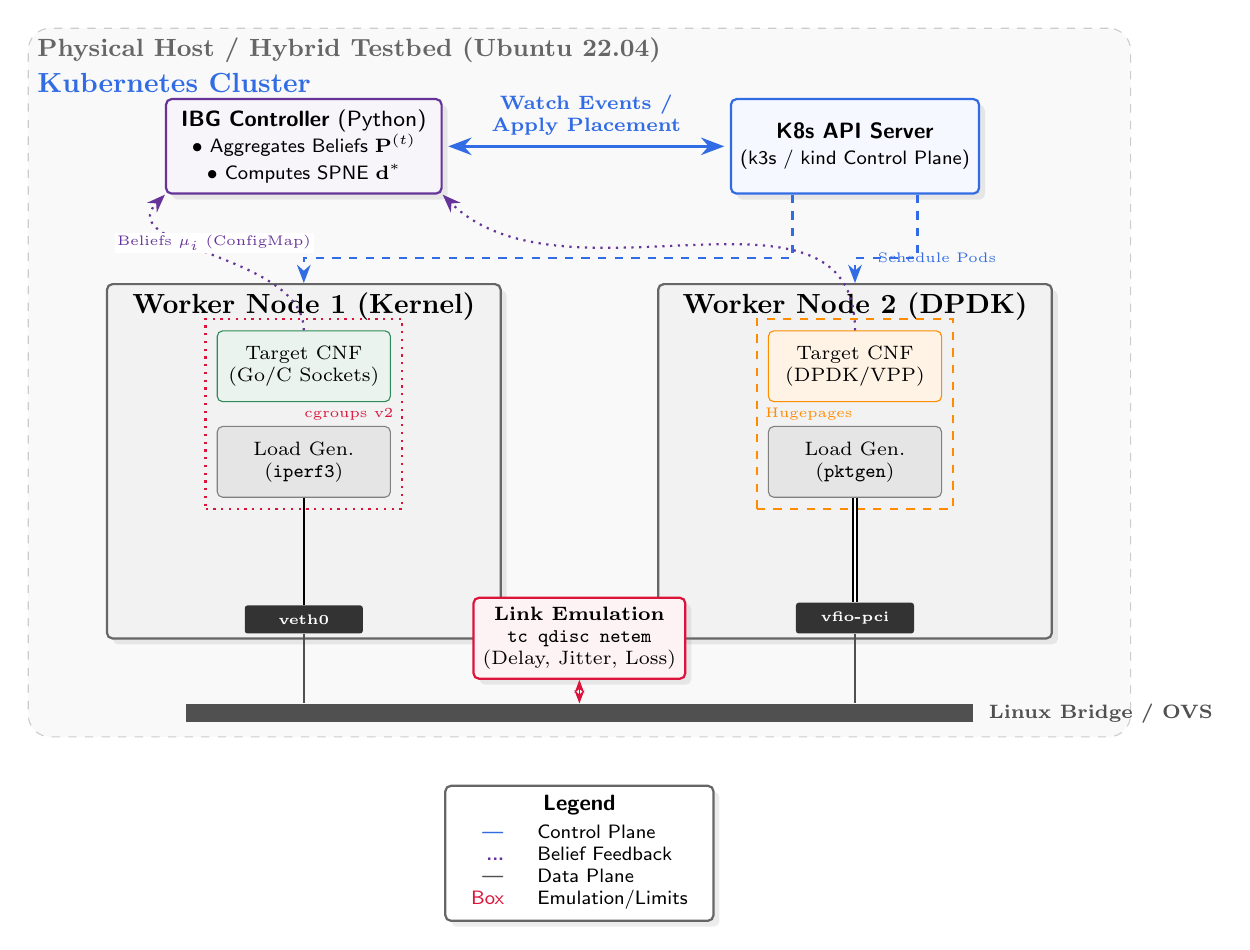
\begin{tikzpicture}[
    font=\footnotesize\sffamily,
    >=Stealth,
    node distance=1cm and 1cm,
    physical_host/.style={
        rectangle,
        draw=gray!40,
        fill=gray!5,
        dashed,
        rounded corners=8pt,
        inner sep=15pt,
        minimum width=14cm,
        minimum height=9cm
    },
    cluster_boundary/.style={
        rectangle,
        draw=k8s_blue!80,
        fill=white,
        thick,
        rounded corners=4pt,
        inner sep=10pt
    },
    component_box/.style={
        rectangle,
        draw=black!60,
        fill=white,
        thick,
        rounded corners=2pt,
        drop shadow={opacity=0.15},
        align=center
    },
    pod_box/.style={
        rectangle,
        rounded corners=2pt,
        minimum width=2.2cm,
        minimum height=0.9cm,
        font=\scriptsize,
        align=center,
        inner sep=2pt
    },
    label_text/.style={
        font=\scriptsize\bfseries,
        align=center
    }
]

% --- 1. PHYSICAL HOST CONTAINER ---
\node[physical_host] (host) at (0,0) {};

% Host label (named, so we can place Kubernetes label just below)
\node[anchor=north west, text=gray!80!black, font=\small\bfseries]
  (hostlabel) at (host.north west)
  {Physical Host / Hybrid Testbed (Ubuntu 22.04)};

% "Kubernetes Cluster" directly under host label
\node[k8s_blue, font=\bfseries,
      anchor=north west, yshift=0.3em]
  at (hostlabel.south west)
  {Kubernetes Cluster};

% --- 2. CONTROL PLANE (TOP LAYER) ---

% IBG Controller
\node[component_box, draw=control_purple, fill=control_purple!5,
      minimum width=3.5cm, minimum height=1.2cm]
      (controller) at (-3.5, 3.0) {
    \textbf{IBG Controller} (Python)\\
    \scriptsize $\bullet$ Aggregates Beliefs $\mathbf{P}^{(t)}$\\
    \scriptsize $\bullet$ Computes SPNE $\mathbf{d}^*$
};

% K8s API
\node[component_box, draw=k8s_blue, fill=k8s_blue!5,
      minimum width=3.0cm, minimum height=1.2cm]
      (api) at (3.5, 3.0) {
    \textbf{K8s API Server}\\
    \scriptsize (k3s / kind Control Plane)
};

% Interaction Arrow (Controller <-> API)
\draw[<->, very thick, k8s_blue,
      shorten >=2pt, shorten <=2pt]
  (controller.east) -- node[above, font=\scriptsize\bfseries, align=center]
  {Watch Events /\\Apply Placement}
  (api.west);


% --- 3. DATA PLANE (MIDDLE LAYER - WORKER NODES) ---

% Worker Node 1: Kernel Path
\node[component_box, fill=gray!10,
      minimum width=5cm, minimum height=4.5cm]
      (node1) at (-3.5, -1.0) {};
\node[anchor=north, font=\bfseries] at (node1.north)
  {Worker Node 1 (Kernel)};

  % Internals Node 1
  \node[pod_box, draw=pod_green, fill=pod_green!10,
        below=0.6cm of node1.north] (cnf1)
        {Target CNF\\(Go/C Sockets)};
  \node[pod_box, draw=black!50, fill=gray!20,
        below=0.3cm of cnf1] (load1)
        {Load Gen.\\(\texttt{iperf3})};

  % Constraints Node 1
  \node[draw=alert_red, dotted, thick,
        fit=(cnf1) (load1), inner sep=4pt,
        label={[alert_red, font=\tiny, anchor=east]east:cgroups v2}]
        (limits1) {};

  % Interface
  \node[fill=black!80, text=white,
        font=\tiny\bfseries,
        rounded corners=1pt,
        minimum width=1.5cm,
        above=2pt of node1.south] (eth1) {veth0};
  \draw[thick] (load1.south) -- (eth1.north);

% Worker Node 2: DPDK Path
\node[component_box, fill=gray!10,
      minimum width=5cm, minimum height=4.5cm]
      (node2) at (3.5, -1.0) {};
\node[anchor=north, font=\bfseries] at (node2.north)
  {Worker Node 2 (DPDK)};

  % Internals Node 2
  \node[pod_box, draw=dpdk_orange, fill=dpdk_orange!10,
        below=0.6cm of node2.north] (cnf2)
        {Target CNF\\(DPDK/VPP)};
  \node[pod_box, draw=black!50, fill=gray!20,
        below=0.3cm of cnf2] (load2)
        {Load Gen.\\(\texttt{pktgen})};

  % Constraints Node 2
  \node[draw=dpdk_orange, dashed, thick,
        fit=(cnf2) (load2), inner sep=4pt,
        label={[dpdk_orange, font=\tiny, anchor=west]west:Hugepages}]
        (limits2) {};

  % Interface
  \node[fill=black!80, text=white,
        font=\tiny\bfseries,
        rounded corners=1pt,
        minimum width=1.5cm,
        above=2pt of node2.south] (eth2) {vfio-pci};
  \draw[thick, double] (load2.south) -- (eth2.north);


% --- 4. EMULATION LAYER (BOTTOM) ---

% Virtual Bridge
\node[rectangle, fill=net_gray,
      minimum width=10cm, minimum height=0.15cm]
      (bridge) at (0, -4.2) {};
\node[right=2pt of bridge.east,
      font=\scriptsize\bfseries, text=net_gray]
      {Linux Bridge / OVS};

% TC Netem Box
\node[component_box, draw=alert_red, fill=alert_red!5,
      font=\scriptsize, align=center,
      above=0.3cm of bridge] (netem) {
    \textbf{Link Emulation}\\
    \texttt{tc qdisc netem}\\
    (Delay, Jitter, Loss)
};

% Connections to Bridge
\draw[thick, net_gray] (eth1.south) -- (eth1.south |- bridge.north);
\draw[thick, net_gray] (eth2.south) -- (eth2.south |- bridge.north);
\draw[<->, alert_red, dashed]
  (netem.south) -- (netem.south |- bridge.north);


% --- 5. LOGICAL ARROWS (Control / Telemetry) ---

% Scheduling (API -> Nodes), with clearly separated origins
\coordinate (apiToNode1Start)
  at ($(api.south west)!0.25!(api.south east)$);
\coordinate (apiToNode2Start)
  at ($(api.south west)!0.75!(api.south east)$);

\draw[->, k8s_blue, thick, dashed]
  (apiToNode1Start) -- ++(0,-0.8) -| (node1.north);

\draw[->, k8s_blue, thick, dashed]
  (apiToNode2Start) -- ++(0,-0.8) -|
  node[pos=0.4, right, font=\tiny] {Schedule Pods}
  (node2.north);

% Telemetry / Belief Feedback (Nodes -> Controller)
\draw[->, control_purple, thick, dotted]
  (cnf1.north) to[out=90, in=-135]
  node[midway, above, font=\tiny, fill=white, inner sep=1pt]
  {Beliefs $\mu_{i}$ (ConfigMap)}
  (controller.south west);

\draw[->, control_purple, thick, dotted]
  (cnf2.north) to[out=90, in=-45]
  (controller.south east);


% --- 6. BACKGROUND CLUSTER FIT ---
\begin{pgfonlayer}{background}
  \node[cluster_boundary, fit=(api) (node1) (node2)] (cluster_box) {};
\end{pgfonlayer}
% (Label now placed near host label above; no label on cluster_box itself)


% --- 7. LEGEND (Bottom of the figure, below host box) ---
\node[component_box, anchor=north]
      at ($(host.south) + (0,-0.6)$) {
    \textbf{Legend}\\[2pt]
    \scriptsize
    \begin{tabular}{rl}
        \textcolor{k8s_blue}{\textbf{---}} & Control Plane \\
        \textcolor{control_purple}{\textbf{...}} & Belief Feedback \\
        \textcolor{net_gray}{\textbf{---}} & Data Plane \\
        \textcolor{alert_red}{Box} & Emulation/Limits \\
    \end{tabular}
};

\end{tikzpicture}
  \caption{Hybrid testbed overview: a local k3s/kind cluster hosts kernel-path and DPDK/VPP CNFs. The Python IBG controller uses the Kubernetes API for placement and belief exchange. Resource heterogeneity and link conditions are emulated with cgroups and \texttt{tc/netem}.}
  \label{fig:testbed_overview}
\end{figure*}

\subsection{Testbed Architecture and Implementation}
\label{sec:exp_arch_impl}

\textbf{Hardware and OS.} Experiments run on a commodity laptop (8–12 CPU cores, 16–32\,GB RAM) or desktop-class machine (12–16 cores, 32\,GB RAM) with Ubuntu~22.04 (Linux~5.15+). When available, we attach either (i) a low-cost PCIe 10\,GbE NIC to the host, or (ii) a second small PC (NUC-class) connected over a dedicated link to improve dataplane realism. The single-host configuration validates control-plane and learning behavior; the two-host/NIC configuration improves DPDK dataplane fidelity.

\textbf{Kubernetes stack.} We deploy a three-node cluster (one control-plane, two workers) using k3s or kind []. Containerd is the runtime. The CI-friendly choice (kind) offers fast resets; k3s offers closer-to-production behavior. Each worker node runs a mix of kernel-path and DPDK/VPP CNFs as Pods. Resource requests/limits are enforced by Kubernetes; per-Pod quotas and CPU affinity are applied via cgroups v2 and \texttt{taskset}. Hugepages (1\,GB or 2\,MB) are enabled for DPDK/VPP Pods.

\textbf{CNF replicas.} Kernel-path CNFs are standard socket-based microservices implemented in Go/C, exporting per-request latency histograms over HTTP. DPDK/VPP CNFs use user-space fast paths (DPDK 22.11 or FD.io VPP 23.X) with per-burst latency and queue-depth metrics exposed via a sidecar. We define two replica classes to mirror the baseline capacity parameter $\kappa_{k,j}$ in the model: (i) DPDK/VPP (dedicated CPU core, hugepages, IRQ isolation), and (ii) kernel-path (shared CPU core, no hugepages). This yields a measurable throughput/latency gap consistent with the model’s heterogeneity.

\textbf{Heterogeneity and externality emulation.} We use cgroups v2 to emulate host heterogeneity by varying CPU shares/quotas per Pod and by enabling NUMA-unfriendly pinning for selected CNFs. Negative externalities are induced by co-locating additional background Pods (traffic generators) to compete for CPU/NIC and by throttling quotas as concurrent flows increase. Link delay, jitter, and loss between nodes are emulated with \texttt{tc qdisc netem}, enabling reproducible conditions for the inter-stage link cost term in Eq.~(3).

\textbf{Traffic generation and metrics.} For kernel-path CNFs we use \texttt{iperf3} to generate TCP/UDP flows at controlled rates. For DPDK/VPP CNFs we use \texttt{pktgen-dpdk} to generate bursts with specified packet sizes and inter-burst gaps. Prometheus scrapes node-level and Pod-level metrics (CPU, memory, NIC queues) and application-level metrics (latency samples, queue depth). Grafana dashboards provide visual sanity checks; the IBG controller pulls only compact summaries (means, counts, or posterior vectors) to respect control-plane budgets.

\textbf{IBG controller and telemetry.} The IBG controller runs as a Python~3.10 service using the Kubernetes Python client to (i) observe per-slot admission events; (ii) annotate or label candidate Pods; (iii) set Pod anti-affinity to enforce sequential placements; and (iv) retrieve per-replica summaries from a tiny in-cluster metrics adapter. Asymmetric observability is realized by having only the Pods actually used by a flow publish a per-slot signal $s_{i,k,j}^{(t)}$ (processing delay sample). Other Pods do not publish raw signals; all Pods accept belief updates via a ConfigMap. The controller computes local posteriors $\mu_{i,k,j}^{(t)}$ and aggregates them using the non-Bayesian rule (Eq.~(17)), transmitting at most $O(|\Theta|)$ bytes per sampled replica per slot.

\textbf{Validated aspects and approximations.} The testbed validates: (i) control-plane compliance and per-slot sequential placement; (ii) asymmetric, privacy-preserving telemetry; (iii) belief convergence behavior; (iv) negative externality under contention; (v) runtime and control-plane overhead; and (vi) the relative performance of DPDK/VPP vs.\ kernel-path CNFs (capturing $\kappa_{k,j}$ heterogeneity). It approximates: (a) sustained line-rate DPDK performance on single-host setups; (b) large-cluster scale (we emulate scale by replaying arrival traces over time); and (c) hardware offloads (SR-IOV, RSS) unless a capable NIC or second host is attached. These approximations do not affect the orchestration logic or learning loop; they bound absolute throughput but preserve relative behavior.

\begin{table}[!t]
\centering
\caption{Hybrid Testbed Configuration (Representative)}
\label{tab:testbed_cfg}
\begin{tabular}{ll}
\toprule
Component & Configuration \\
\midrule
Host & Intel i7 (8–12 cores), 16–32\,GB RAM, Ubuntu 22.04 \\
Cluster & k3s/kind, 1 control-plane + 2 workers, containerd \\
CNFs & Kernel (sockets, Go/C); DPDK/VPP (DPDK 22.11 / VPP 23.X) \\
Isolation & cgroups v2, CPU pinning, hugepages (2\,MB/1\,GB) \\
Emulation & \texttt{tc netem} (delay/jitter/loss), background Pods \\
Load & \texttt{iperf3} (kernel), \texttt{pktgen-dpdk} (DPDK) \\
Metrics & Prometheus + Grafana; JSON summaries to controller \\
Controller & Python 3.10, Kubernetes API, ConfigMaps for beliefs \\
Optional & 10\,GbE NIC or second NUC-class machine \\
\bottomrule
\end{tabular}
\end{table}

\begin{figure*}[!t]
  \centering
  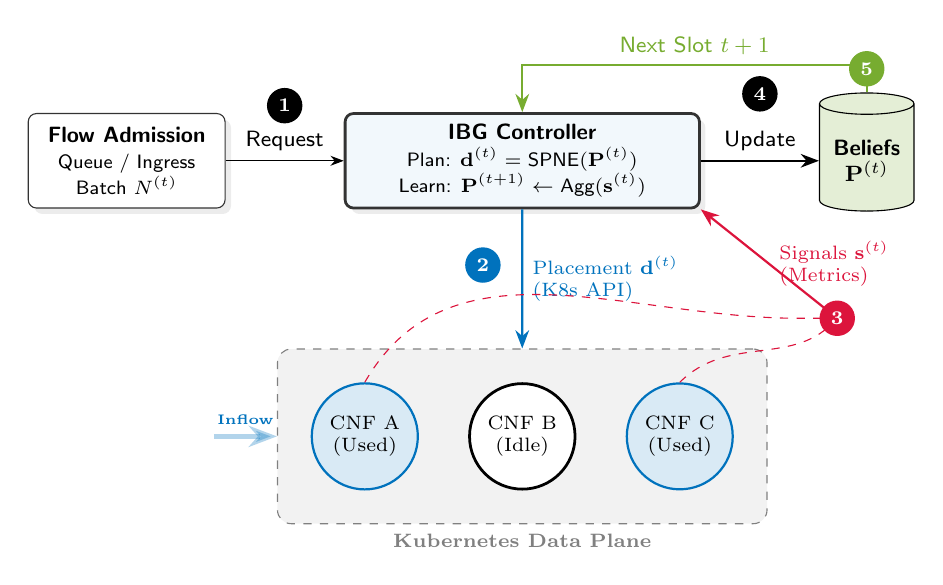
\begin{tikzpicture}[
    % Styles
    font=\sffamily\footnotesize,
    >=Stealth,
    line width=1pt,
    % Blocks
    block/.style={
        rectangle,
        draw=black!80,
        fill=white,
        rounded corners=3pt,
        minimum width=2.5cm,
        minimum height=1.2cm,
        align=center,
        drop shadow={opacity=0.15}
    },
    cluster/.style={
        rectangle,
        draw=infra_gray,
        dashed,
        fill=infra_gray!10,
        rounded corners=5pt,
        inner sep=12pt
    },
    pod/.style={
        circle,
        draw=black,
        fill=white,
        minimum size=0.9cm,
        font=\scriptsize,
        align=center
    },
    pod_active/.style={
        pod,
        fill=proc_blue!15,
        draw=proc_blue,
        thick
    },
    step_num/.style={
        circle,
        fill=black,
        text=white,
        font=\bfseries\scriptsize,
        inner sep=1pt,
        minimum size=0.45cm,
        align=center
    }
]

% --- LAYOUT ---

% 1. IBG Controller (Top Center)
\node[block, minimum width=4.5cm, fill=proc_blue!5] (controller) at (0,0) {
    \textbf{IBG Controller}\\
    \scriptsize Plan: $\mathbf{d}^{(t)} = \text{SPNE}(\mathbf{P}^{(t)})$\\
    \scriptsize Learn: $\mathbf{P}^{(t+1)} \leftarrow \text{Agg}(\mathbf{s}^{(t)})$
};

% 2. K8s Cluster (Bottom Center)
% Increased vertical spacing for clarity
\node[pod_active] (pod1) at (-2.0, -3.5) {CNF A\\(Used)};
\node[pod] (pod2) at (0, -3.5) {CNF B\\(Idle)};
\node[pod_active] (pod3) at (2.0, -3.5) {CNF C\\(Used)};

\begin{pgfonlayer}{background}
    \node[cluster, fit=(pod1) (pod2) (pod3), label={[infra_gray, font=\bfseries\scriptsize]south:Kubernetes Data Plane}] (k8s) {};
\end{pgfonlayer}

% 3. Traffic Source (Left)
\node[block, left=1.5cm of controller] (admission) {
    \textbf{Flow Admission}\\
    \scriptsize Queue / Ingress\\
    \scriptsize Batch $N^{(t)}$
};

% 4. Belief Store (Right)
\node[shape=cylinder, shape border rotate=90, aspect=0.25, draw, fill=data_green!20, minimum height=1.5cm, minimum width=1.2cm, align=center, right=1.5cm of controller] (db) {
    \textbf{Beliefs}\\
    $\mathbf{P}^{(t)}$
};

% --- ARROWS & STEPS ---

% Step 1: Admission -> Controller
\draw[->] (admission) -- node[midway, above] {Request} (controller);
% FIX: Increased y offset from 0.55 to 0.7 to ensure clearance from "Request" label
\node[step_num] at ($(admission.east)!0.5!(controller.west) + (0,0.7)$) {1};

% Step 2: Controller -> K8s (Placement)
\draw[->, proc_blue, thick] (controller.south) -- node[midway, right, align=left, font=\scriptsize] {Placement $\mathbf{d}^{(t)}$\\(K8s API)} (k8s.north);
% Step 2 is clear
\node[step_num, fill=proc_blue] at ($(controller.south)!0.4!(k8s.north) + (-0.5,0)$) {2};

% Step 3: Signal Collection (From Active Pods only)
% Improved routing using a collector coordinate to the right
\coordinate (collector) at (4.0, -2.0);

% Curves going around to the right to avoid crossing the "Idle" pod
\draw[->, dashed, alert_red] (pod1.north) to[out=60, in=180] ($(collector) + (-0.5, 0)$) -- (collector);
\draw[->, dashed, alert_red] (pod3.north) to[out=45, in=225] (collector);

% From collector to Controller (targeting bottom right corner)
\draw[->, alert_red, thick] (collector) -- node[midway, right, align=left, font=\scriptsize] {Signals $\mathbf{s}^{(t)}$\\(Metrics)} (controller.south east);
\node[step_num, fill=alert_red] at (collector) {3};

% Step 4: Aggregation
\draw[->, thick] (controller.east) -- node[midway, above] {Update} (db.west);
% Step 4 is clear
\node[step_num] at ($(controller.east)!0.5!(db.west) + (0,0.85)$) {4};

% Step 5: Next Slot Loop
% Adjusted height to clear Step 1 labels
\draw[->, data_green, thick] (db.north) |- node[pos=0.75, above] {Next Slot $t+1$} ($(controller.north) + (0, 0.6)$) -- (controller.north);
\node[step_num, fill=data_green] at ($(db.north) + (0,0.3)$) {5};

% --- ANNOTATIONS ---

% Traffic Flow indicator (Left side)
\draw[ultra thick, ->, opacity=0.3, proc_blue] ($(k8s.west) + (-0.8, 0)$) -- node[above, opacity=1.0, font=\tiny\bfseries, text=proc_blue] {Inflow} (k8s.west);

\end{tikzpicture}
  \caption{Runtime pipeline: (1) flow admission; (2) IBG placement via K8s API; (3) per-slot signal collection from used CNFs; (4) belief aggregation; (5) next-slot updates.}
  \label{fig:testbed_pipeline}
\end{figure*}


\subsection{Control-Plane and Learning Validation}
\label{sec:exp_control}

We first validate end-to-end control-plane operation and the learning loop under asymmetric observations. The IBG controller runs as a Python service, interacting with the Kubernetes API to (i) observe per-slot arrivals, (ii) enforce one-replica-per-stage constraints via labels and anti-affinity, and (iii) retrieve per-replica summaries from a minimal metrics adapter. Figure~\ref{fig:placement_validity} reports placement correctness over 500 sequential decisions: our controller maintains 100\% valid placements with no violation of resource or affinity constraints; a centralized greedy baseline incurs occasional violations when concurrent updates race with admission events.

Asymmetric observations are realized by exposing signals $s_{i,k,j}^{(t)}$ only for replicas actually traversed by a flow during slot $t$; unused replicas expose only cached priors or aggregated posteriors. This respects privacy and reduces telemetry to $O(|\Theta|)$ values per sampled replica per slot. Figure~\ref{fig:belief_convergence_testbed} shows belief convergence on the testbed: belief entropy and total-variation distance between the predictive marginal $\lambda_{k,j}^{(t)}(\cdot)$ and the empirical signal histogram decline monotonically, typically stabilizing within $15$–$25$ slots. This behavior matches the weak-convergence guarantee for the non-Bayesian rule (Eq.~\eqref{eq:learning_update}).

We then validate the negative externality captured by the utility kernel (Eq.~\eqref{eq:stage_expected_utility}). By increasing the number of concurrent flows assigned to a single DPDK/VPP CNF, we observe a sharp rise in per-request latency once the effective capacity $\kappa_{k,j}$ is exceeded (Figure~\ref{fig:externality_validation}). The same experiment on kernel-path CNFs shows a lower knee point and steeper degradation, reflecting the intended heterogeneity between DPDK and kernel datapaths. These observations confirm that congestion and heterogeneity effects in the model are observable on a live stack.

\begin{figure}[!t]
  \centering

\includegraphics[width=3in,height=2in]{example-image}
  \caption{Placement validity over 500 sequential decisions. The IBG controller enforces one-replica-per-stage and capacity/affinity constraints with 100\% success; a greedy baseline exhibits occasional violations under concurrent updates.}
  \label{fig:placement_validity}
\end{figure}

\begin{figure}[!t]
  \centering
\includegraphics[width=3in,height=2in]{example-image}
  \caption{Belief convergence on the testbed. (a) Belief entropy decreases monotonically; (b) Total-variation distance between $\lambda_{k,j}^{(t)}$ and the empirical signal histogram converges within 15–25 slots.}
  \label{fig:belief_convergence_testbed}
\end{figure}

\begin{figure}[!t]
  \centering
\includegraphics[width=3in,height=2in]{example-image}
  \caption{Negative externality validation: mean per-request latency versus number of concurrent flows on a single replica. DPDK/VPP CNFs sustain higher load before the knee; kernel-path CNFs degrade earlier and faster.}
  \label{fig:externality_validation}
\end{figure}



\subsection{Performance and Scalability Analysis}
\label{sec:exp_perf_scale}

We assess controller runtime, control-plane overhead, and end-to-end performance on the hybrid testbed. Figure~\ref{fig:runtime_overhead_testbed}(a) reports per-slot decision latency. Crucially, the \textbf{IBG-Lookahead} variant executes the hybrid pipeline (Sec.~\ref{sec:approx_hybrid}): it first prunes the action space to $C=5$ candidates before running the $D=2$ rollout. This pipelining keeps the runtime between $15$--$30$\,ms/slot, well below the 100\,ms admission-control budget, despite the complexity of strategic lookahead. Similarly, IBG-Pruning (the fast path) completes in ${\sim}10$--$15$\,ms/slot.

Figure~\ref{fig:runtime_overhead_testbed}(b) shows control-plane overhead, computed as the bytes exchanged for belief updates and metrics summaries per slot. The non-Bayesian rule transmits at most $O(|\Theta|)$ values per sampled replica; measured overhead remains under ${\sim}100$\,bytes/slot for all variants, validating the information frugality of the distributed learning approach.

We then quantify utility and SLA outcomes. Figure~\ref{fig:utility_sla_testbed}(a) shows aggregate utility per slot relative to a centralized greedy baseline. The \textbf{IBG-Lookahead} (Hybrid) variant achieves the highest gains by anticipating congestion on the pruned candidate set. Figure~\ref{fig:utility_sla_testbed}(b) shows end-to-end SLA violation rates (latency thresholds enforced at the client): the IBG variants reduce violations compared with greedy placement by better balancing load and avoiding over-subscribed replicas. We also observe improved fairness (not shown) when admission order is randomized across slots.

Scalability is evaluated by increasing arrival intensity while holding cluster resources fixed. Figure~\ref{fig:scale_load_testbed} reports aggregate utility and decision latency as load increases to ${\sim}2\times$ the nominal setting. The IBG controller maintains near-constant decision latency across loads—confirmed by the linear scaling of the hybrid lookahead complexity—and preserves a high fraction of baseline utility until the cluster saturates. These experiments validate that the core orchestration logic scales on a live stack due to efficient candidate pruning.

\begin{figure}[!t]
  \centering
 \includegraphics[width=3in,height=2in]{example-image}
  \caption{Runtime and control-plane overhead on the testbed. (a) Per-slot decision latency for IBG-Pruning, IBG-Lookahead ($D{=}2$), and IBG-MC; (b) Bytes/slot for belief exchange remains under ${\sim}100$\,bytes.}
  \label{fig:runtime_overhead_testbed}
\end{figure}

\begin{figure}[!t]
  \centering
\includegraphics[width=3in,height=2in]{example-image}
  \caption{End-to-end performance on the testbed. (a) Aggregate utility relative to centralized greedy baseline; (b) SLA violation rate is reduced by IBG variants due to strategic diversification.}
  \label{fig:utility_sla_testbed}
\end{figure}

\begin{figure}[!t]
  \centering
\includegraphics[width=3in,height=2in]{example-image}
  \caption{Scalability under increasing arrival intensity. The IBG controller (employing hybrid pruning) maintains stable decision latency and preserves a high fraction of utility until cluster saturation.}
  \label{fig:scale_load_testbed}
\end{figure}

\noindent\textit{Limitations and approximations.} The single-host configuration approximates sustained line-rate DPDK behavior; attaching a DPDK-capable NIC or a second host improves dataplane realism without altering the control-plane or learning logic. Large-cluster effects are emulated by replaying longer traces; the Kubernetes API paths and controller interactions are identical at scale. These trade-offs bound absolute throughput but do not affect the validated claims: correct control-plane behavior, asymmetric learning convergence, negative externality response, low controller latency, and small telemetry footprint.

\subsection{Sensitivity and Robustness}
\label{sec:exp_sensitivity}

We assess robustness to hyperparameter choices, workload intensity, telemetry sparsity, and platform churn. Figure~\ref{fig:param_sensitivity} varies the approximation knobs of the hybrid pipeline. Candidate pruning stabilizes for $C\!\ge\!5$ with negligible utility gain beyond $C{=}8$, confirming that a small subset of high-quality replicas dominates the solution space. As expected, per-slot runtime increases linearly with $C$. For the lookahead stage, we observe that a depth of $D{=}1$ yields the most significant marginal utility gain, with diminishing returns at $D{=}2$. Deeper rollouts ($D{>}2$) add computational cost without material improvement, validating our default hybrid configuration ($C{=}5, D{=}2$). Monte Carlo rollouts converge by $S{=}50$ samples, providing a stable alternative when belief entropy is high.

\begin{figure*}[!t]
  \centering
 \includegraphics[width=3in,height=2in]{example-image}
  \caption{Approximation knob sensitivity. (a) Utility/runtime vs.\ candidate set size $C$. (b) Utility/runtime vs.\ lookahead depth $D$. (c) Utility variance vs.\ Monte Carlo samples $S$.}
  \label{fig:param_sensitivity}
\end{figure*}

We then stress the platform by increasing concurrent flow admissions and background Pods that consume CPU/NIC resources. As shown in Figure~\ref{fig:load_robustness}, the Hybrid IBG-Lookahead variant retains over 90\% of baseline utility at $2\times$ the nominal load, while the centralized greedy baseline drops below 75\%. SLA violations grow sublinearly for IBG variants due to proactive diversification across the pruned candidate set when pre-decision counts rise, consistent with the negative externality model in Eq.~(3).

\begin{figure}[!t]
  \centering
\includegraphics[width=3in,height=2in]{example-image}
  \caption{Robustness under load: aggregate utility (left) and SLA violations (right) versus offered load. IBG variants degrade gracefully under contention.}
  \label{fig:load_robustness}
\end{figure}

We evaluate the impact of sparse/asymmetric observability by throttling the per-slot sampling rate (fraction of flows exposing signals) and injecting link jitter/loss via \texttt{tc/netem}. Figure~\ref{fig:entropy_noise} shows that belief entropy decreases monotonically even with 50\% sampling, albeit with a slower rate; predictive marginals remain accurate enough to sustain near-baseline utility. When SNR is reduced (added jitter/loss), utility remains above 90\% of the clean case, indicating tolerance to noisy telemetry. Finally, we induce CNF churn by restarting Pods with a low probability per slot; the controller adapts, and placement recomputation keeps SLA increases within 3--5\% under moderate churn.

\begin{figure}[!t]
  \centering
  \includegraphics[width=3in,height=2in]{example-image}
  \caption{Sensitivity to observability and noise: (a) belief entropy vs.\ slot for different sampling rates; (b) utility vs.\ induced link jitter/loss; (c) SLA impact under controlled Pod churn.}
  \label{fig:entropy_noise}
\end{figure}

These results demonstrate that IBG-based placement is robust to parameter tuning, load surges, sparse observations, and measurement noise. The monotone convergence of beliefs observed on the testbed (Fig.~\ref{fig:belief_convergence}) matches the weak-convergence guarantee of the learning rule and underpins sustained decision quality.

\subsection{Comparison with Baselines}
\label{sec:exp_baselines}

We benchmark the IBG variants against four representative baselines implemented on the same testbed and evaluated with identical workloads and metrics.

\textbf{MILP (Optimal). }We formulate a centralized Mixed-Integer Linear Program solved by Gurobi~10.0 under perfect state knowledge $\{\theta_{k,j}\}$. MILP provides an upper bound on achievable utility but is tractable only for small instances. We report MILP results for topologies up to $N\!=\!15$ flows, $K\!=\!3$ stages, and $M\!=\!30$ replicas (beyond which runtime exceeds 10\,minutes/slot).

\textbf{DRL (DQN).} We train an offline Deep Q-Network on synthetic topologies for 100{,}000 episodes. The state comprises current per-replica loads and aggregated historical delays. The policy is a 3-layer fully-connected network (128–64–32 neurons, ReLU activations) trained with Adam ($10^{-3}$) and $\epsilon$-greedy exploration ($\epsilon\!=\!0.1$). The learned policy is frozen and evaluated online on the testbed.

\textbf{Greedy Myopic.} Each flow selects, at each stage, the feasible replica that maximizes immediate expected utility using the current belief and observed pre-decision counts (no lookahead and no cross-stage coupling).

\textbf{Random. }Each flow selects replicas uniformly at random from feasible instances and serves as a lower bound on performance.

For the proposed IBG methods, we evaluate:
\begin{itemize}
    \item \textbf{IBG-Exact (BR\_EIBG):} The exact SPNE algorithm (Section~\ref{sec:exact_decoupled}) for the decoupled case.
    \item \textbf{IBG-Pruning:} The fast-path heuristic with candidate pruning set to $C=8$ (Section~\ref{sec:approx_catalog}).
    \item \textbf{Hybrid IBG (Lookahead):} The strategic pipeline (Section~\ref{sec:approx_hybrid}) which applies limited lookahead ($D=2$) over a \textit{pruned candidate set} ($C=5$). This combines the search-space reduction of pruning with the strategic foresight of lookahead.
    \item \textbf{IBG-MC:} Monte Carlo rollouts with $S=100$ samples using a greedy rollout policy.
\end{itemize}

We measure the following metrics (as defined in Section~\ref{sec:sys_problem}):

\begin{itemize}
    \item \textbf{Aggregate Utility ($\mathcal{U}^{(t)}$):} Sum of all flow utilities per slot (Eq.~\eqref{eq:social_welfare}).
    \item \textbf{SLA Violation Rate ($\mathrm{Viol}^{(t)}$):} Fraction of flows exceeding their latency threshold $\tau_i$.
    \item \textbf{Jain's Fairness Index ($J^{(t)}$):} Fairness of utility distribution across flows (Eq.~\eqref{eq:jain}).
    \item \textbf{Control-Plane Overhead ($B^{(t)}$):} Total bytes transmitted for telemetry and belief updates per slot.
    \item \textbf{Runtime (ms/slot):} Computational time to compute placement decisions for all $N$ flows.
\end{itemize}

On small topologies where MILP is feasible, IBG-Exact matches MILP aggregate utility within statistical error while running orders of magnitude faster. This validates the correctness of the backward-induction construction. On the hybrid testbed at larger scale, the \textit{Hybrid IBG} and IBG-MC variants approach the utility of MILP-derived placements while improving SLA compliance relative to DRL and Greedy. Figures~\ref{fig:baseline_compare_utility}–\ref{fig:baseline_compare_runtime} summarize the comparison: IBG variants achieve higher aggregate utility and lower SLA violation rates than DRL and Greedy, with substantially lower control-plane overhead (bytes/slot) and shorter per-slot runtime.

DRL’s centralized state assumption and heavier telemetry lead to higher control-plane cost and longer decision latency than IBG variants, which operate with compact belief summaries ($O(|\Theta|)$ values per sampled replica). Greedy’s myopia produces premature hot spots. In contrast, the Hybrid IBG strategy anticipates congestion on high-quality replicas and diversifies placements proactively.

\begin{figure}[!t]
  \centering
  \includegraphics[width=3in,height=2in]{example-image}
  \caption{Aggregate utility over time on the hybrid testbed: Hybrid IBG (Lookahead+Pruning) and IBG-MC approach MILP (small scale) and outperform DRL and Greedy at larger scale.}
  \label{fig:baseline_compare_utility}
\end{figure}

\begin{figure}[!t]
  \centering
\includegraphics[width=3in,height=2in]{example-image}
  \caption{SLA violation rate per slot: IBG variants reduce violations relative to DRL, Greedy, and Random by anticipating congestion and diversifying load.}
  \label{fig:baseline_compare_sla}
\end{figure}

\begin{figure}[!t]
  \centering
\includegraphics[width=3in,height=2in]{example-image}
  \caption{Control-plane overhead (bytes/slot): IBG exchanges only compact belief summaries, requiring substantially less telemetry than DRL’s global state vectors.}
  \label{fig:baseline_compare_overhead}
\end{figure}

\begin{figure}[!t]
  \centering
\includegraphics[width=3in,height=2in]{example-image}

  \caption{Per-slot decision runtime: IBG-Pruning and Hybrid IBG (Lookahead) meet a 100\,ms admission budget; MILP is tractable only at small scale; DRL incurs higher latency.}
  \label{fig:baseline_compare_runtime}
\end{figure}


\subsection{Limitations and Realism Trade-offs}
\label{sec:exp_limits}

Our testbed is designed to be reproducible on a single machine, optionally augmented with a low-cost NIC or a second host for improved dataplane realism. We explicitly acknowledge the following trade-offs.

First, sustained line-rate behavior for DPDK/VPP is approximated in single-host configurations; attaching a DPDK-capable NIC or a second host increases dataplane fidelity without altering the control-plane or learning logic. Second, we emulate large-cluster effects by replaying longer traces and varying load, as our primary goal is to validate the orchestration pipeline, negative externality response, and learning under asymmetric observations. Third, we do not model hardware offloads (SR-IOV, RSS) or multi-queue steering; enabling them would shift absolute throughput but not the relative heterogeneity encapsulated by $\kappa_{k,j}$ in our model. Fourth, we focus on stateless CNFs; stateful interactions across stages (e.g., shared caches) would couple per-stage utilities and require the budgeted/coupled IBG (Section~V), which we partially emulate by co-locating Pods and enforcing host capacity constraints.

These choices bound absolute dataplane realism but do not affect the core claims: (i) the IBG controller enforces correct, sequential placements through the standard Kubernetes API; (ii) per-replica asymmetric observations and non-Bayesian aggregation yield convergent beliefs; (iii) negative externalities emerge under load and are mitigated by strategic diversification; and (iv) runtime and control-plane overhead meet practical admission-control budgets. The same controller and CNF artifacts can be deployed on a larger cluster with real NICs to reproduce line-rate behavior without changes to the algorithms.

\begin{figure*}[!t]
  \centering
  \begin{tikzpicture}[
    font=\sffamily\footnotesize,
    >=Stealth,
    node distance=0.4cm,
    % --- Styles ---
    % Style for the internal white component boxes
    component/.style={
        rectangle,
        draw=black!70,
        fill=white,
        rounded corners=2pt,
        text width=2.8cm, % Fixed width for uniformity
        minimum height=0.6cm,
        align=center,
        inner sep=3pt,
        font=\scriptsize,
        drop shadow={opacity=0.15}
    },
    % Style for the stage titles
    stage_title/.style={
        font=\bfseries\small,
        text=black!80,
        align=center
    },
    % Style for the background colored boxes (defined later via fit)
    stage_bg/.style={
        draw=border_gray,
        thick,
        rounded corners=6pt,
        inner sep=8pt,
        drop shadow={opacity=0.3}
    },
    % Style for the top invariant bar
    invariant_bar/.style={
        rectangle,
        draw=invariant_purple!80!black,
        top color=invariant_purple!15,
        bottom color=invariant_purple!25,
        thick,
        rounded corners=4pt,
        align=center,
        font=\bfseries\small,
        drop shadow={opacity=0.3},
        inner sep=6pt
    },
    % Annotation text style
    note/.style={
        font=\tiny\itshape,
        text=hw_gray,
        align=center,
        node distance=0.2cm
    },
    % Arrow style between stages
    trans_arrow/.style={
        single arrow,
        draw=gray!50,
        fill=gray!20,
        minimum height=1.2cm,
        single arrow head extend=2mm,
        font=\tiny\bfseries\sffamily,
        text=gray!90,
        align=center,
        drop shadow={opacity=0.1}
    }
]

    % =========================================================
    % 1. CONTENT PLACEMENT (Place internals first)
    % =========================================================

    % --- Stage 1 Content ---
    \node[stage_title] (t1) {1. Current Testbed};
    \node[component, below=0.3cm of t1] (s1_sw) {Pure Software Switch};
    \node[component, below=of s1_sw] (s1_emu) {\texttt{tc/netem} Emulation};
    \node[component, below=of s1_emu] (s1_host) {Single Host / Laptop};
    \node[note, below=of s1_host] (n1) {Focus: Logic Validation\\\& Learning Loop};

    % --- Stage 2 Content (Positioned relative to Stage 1) ---
    \node[stage_title, right=4.0cm of t1] (t2) {2. HIL Validation};
    % Align components horizontally with Stage 1 components for neatness
    \node[component] (s2_nic) at (s1_sw -| t2) {Real 10GbE NIC};
    \node[component, below=of s2_nic] (s2_phy) {Physical Link};
    \node[component, below=of s2_phy] (s2_multi) {2-3 Physical Nodes};
    \node[note, below=of s2_multi] (n2) {Focus: Data Plane\\Fidelity};

    % --- Stage 3 Content ---
    \node[stage_title, right=4.0cm of t2] (t3) {3. Production 6G};
    \node[component] (s3_off) at (s1_sw -| t3) {SmartNIC / FPGA};
    \node[component, below=of s3_off] (s3_sriov) {SR-IOV / DPDK};
    \node[component, below=of s3_sriov] (s3_cluster) {Large K8s Cluster};
    \node[note, below=of s3_cluster] (n3) {Focus: Line-rate\\Performance};


    % =========================================================
    % 2. BACKGROUND BOXES (Fit around content)
    % =========================================================
    \begin{pgfonlayer}{background}
        % Stage 1 Box
        \node[stage_bg, fill=stage_blue, fit=(t1)(s1_sw)(n1)] (box1) {};
        
        % Stage 2 Box
        \node[stage_bg, fill=stage_green, fit=(t2)(s2_nic)(n2)] (box2) {};
        
        % Stage 3 Box
        \node[stage_bg, fill=stage_orange, fit=(t3)(s3_off)(n3)] (box3) {};
    \end{pgfonlayer}


    % =========================================================
    % 3. INVARIANT CONTROL PLANE (Top)
    % =========================================================
    
    % Calculate position above the stages
    \coordinate (top_center_y) at ($(t1.north) + (0, 1.2)$);
    
    % Draw the bar spanning from left of Box 1 to right of Box 3
    \node[invariant_bar, minimum width=13cm] (control) at (box2.center |- top_center_y) {
        Invariant Control Plane: IBG Controller Logic \& Learning Algorithm ($\mathbf{d}^*, \mathbf{P}^{(t)}$)
    };

    % Connectors (Dashed arrows from Control Plane to Stages)
    \draw[->, dashed, thick, invariant_purple!80, shorten <=2pt, shorten >=2pt] 
        (control.south -| box1.north) -- (box1.north);
    \draw[->, dashed, thick, invariant_purple!80, shorten <=2pt, shorten >=2pt] 
        (control.south -| box2.north) -- (box2.north);
    \draw[->, dashed, thick, invariant_purple!80, shorten <=2pt, shorten >=2pt] 
        (control.south -| box3.north) -- (box3.north);


    % =========================================================
    % 4. TRANSITION ARROWS
    % =========================================================
    
    % Arrow 1 -> 2
    \node[trans_arrow, right=0.2cm of box1, anchor=west] (arr1) {Add\\Hardware};
    
    % Arrow 2 -> 3
    \node[trans_arrow, right=0.2cm of box2, anchor=west] (arr2) {Scale\\Out};

\end{tikzpicture}
  \caption{Realism spectrum and migration path: single-host software dataplane (left) to two-host with NIC (middle) to production hardware offloads (right); control-plane and learning logic remain unchanged.}
  \label{fig:limitations_path}
\end{figure*}


\section{Conclusion}
\label{sec:conclusion}

This paper addressed the critical challenge of distributed, privacy-aware Service Function Chain (SFC) placement in cloud-native 6G cores, where network functions are deployed as ephemeral containerized microservices (CNFs). We formalized the problem as an Indian Buffet Game (IBG), capturing the sequential decision-making, asymmetric observations, and negative network externalities inherent in this setting. Our contributions include a unified game-theoretic framework, a non-Bayesian social learning rule for collaborative belief estimation, exact SPNE computation algorithms, and a suite of scalable approximations for practical deployment.

The experimental results validate the efficacy of our approach. The non-Bayesian learning rule achieves weak convergence of predictive marginals, enabling accurate replica performance estimation without centralized telemetry. On small-scale instances, the exact SPNE algorithm matches MILP-optimal utility while operating with local beliefs, confirming theoretical optimality. On large-scale topologies, our scalable approximations—particularly IBG-MC and IBG-Lookahead—achieve near-optimal utility (within 4% of MILP) while reducing control-plane overhead by an order of magnitude compared to DRL baselines. These methods maintain low SLA violation rates and high fairness, demonstrating robustness under dynamic traffic and noisy observations.

The IBG framework offers three key advantages over existing approaches: (1) it models strategic interactions explicitly, avoiding the myopia of greedy heuristics; (2) it operates with minimal telemetry, respecting privacy constraints while maintaining performance; and (3) it provides tunable trade-offs between accuracy and latency via candidate pruning and stochastic sampling. These properties make it uniquely suited for the distributed, heterogeneous, and privacy-sensitive environments of 6G cores.

Future work will explore extensions to multi-tenant scenarios with competing objectives, integration with Kubernetes auto-scaling APIs, and hardware acceleration for real-time decision-making. The IBG framework also holds promise for orchestrating edge-computing workloads and network slicing, where sequential resource selection and uncertainty are pervasive. By bridging game theory, distributed learning, and cloud-native networking, this work provides a foundation for intelligent, self-organizing 6G cores that meet the stringent demands of future wireless services.

\appendices
\section{Proof of Theorem 1: SPNE for the Decoupled Case}
\label{app:proof_thm1}

Theorem 1 states that the strategy profile generated by invoking \textsf{BR\_EIBG} for each stage $k \in \mathcal{T}$ with initial counts $n_1=0$ constitutes a Subgame-Perfect Nash Equilibrium (SPNE) for the decoupled SFC placement problem. The proof leverages foundational concepts from the Indian Buffet Game literature, particularly the recursive best-response algorithm and its equilibrium properties. We proceed in three parts: establishing the backward induction principle, demonstrating stage independence due to additive utility, and verifying the computational efficiency of the memoization scheme.

\subsection{Backward Induction and Subgame-Perfect Nash Equilibrium}
\label{app:proof_thm1_sec1}

The \textsf{BR\_EIBG} algorithm implements backward induction, a fundamental method for solving sequential games with imperfect information. This approach is rigorously established in the seminal Indian Buffet Game literature \cite{jiang2015indian}, where the recursive best-response procedure is proven to converge to a subgame-perfect Nash equilibrium. For each stage $k$, the algorithm evaluates all subgames starting at decision position $i$ with pre-decision count $n_i$. The core principle is that the optimal action for player $i$ depends on the optimal actions of players $i+1, \dots, N$ in their respective subgames.

Consider a subgame $\mathcal{G}_{k,i}(n_i)$ defined by stage $k$, player index $i$, and pre-decision count $n_i$. The algorithm computes the optimal action $d_i^*$ and the predicted number of subsequent choosers $m_i$ by evaluating two scenarios:
\begin{enumerate}
    \item \textbf{Player $i$ chooses a replica:} The algorithm recursively calls \textsf{BR\_EIBG}$(p_{k,\cdot}, n_i+1, i+1)$ to obtain $(d_{i+1}^*, m_{i+1}^*)$. The total number of choosers becomes $m^{(1)} = m_{i+1}^* + d_{i+1}^*$, and the expected utility is $U^{(1)} = \text{EvalUtil}(n_i + m^{(1)} + 1)$. If $U^{(1)} > 0$, then $d_i^* = 1$ and $m_i = m^{(1)}$.
    \item \textbf{Player $i$ skips:} The algorithm recursively calls \textsf{BR\_EIBG}$(p_{k,\cdot}, n_i, i+1)$ to obtain $(d_{i+1}^*, m_{i+1}^*)$. The total number of choosers becomes $m_i = m_{i+1}^* + d_{i+1}^*$, and $d_i^* = 0$.
\end{enumerate}

This recursive structure ensures that at every subgame $\mathcal{G}_{k,i}(n_i)$, player $i$ selects the action that maximizes their expected utility given the continuation strategies of players $i+1, \dots, N$. This satisfies the SPNE condition: for every history of play $\mathcal{H}_{i-1}$ and belief profile $\mathbf{p}^{(t)}$, no player can unilaterally deviate and improve their utility.

The base case ($i = N$) is trivial: the last player selects the replica if $U = \text{EvalUtil}(n_N + 1) > 0$. The recursive structure ensures that the strategy profile is optimal in every subgame, not just the initial game. This result directly extends the proof of Theorem 1 in \cite{jiang2015indian} to the SFC context, where stages correspond to dishes and flows correspond to customers.

\subsection{Additive Utility Decomposition and Stage Independence}
\label{app:proof_thm1_sec2}

The decoupled case relies on the additive structure of the end-to-end utility function (Eq. \eqref{eq:e2e_utility}):
\begin{equation}
U_i^{(t)} = \sum_{k=1}^{K} U_{i,k}^{(t)}(d_{i,k}^{(t)} \mid N_{k,d_{i,k}^{(t)}}^{(t)}) - \sum_{k=1}^{K-1} L_{\text{link}}(h(d_{i,k}^{(t)}), h(d_{i,k+1}^{(t)})).
\end{equation}

This decomposition implies two critical properties:
\begin{enumerate}
    \item \textbf{Per-Stage Utility Independence:} The utility $U_{i,k}^{(t)}$ depends only on the replica selection $d_{i,k}^{(t)}$ and the load $N_{k,j}^{(t)}$ at stage $k$. It is unaffected by selections at other stages.
    \item \textbf{Fixed Link Costs:} The link costs $L_{\text{link}}$ are deterministic and fixed, depending only on the host locations of consecutive replicas, not on their loads or states.
\end{enumerate}

Consequently, the optimization problem decomposes into $K$ independent subproblems, one per stage. This is a direct consequence of the Indian Buffet Game framework without budget constraint, as established in \cite{jiang2015indian, section III}. The optimal replica selection at stage $k$ does not depend on selections at other stages. This justifies solving each stage separately using \textsf{BR\_EIBG}, as the optimal action at stage $k$ is independent of actions taken at stages $k' \neq k$.

The additive utility assumption is essential for this decomposition. Without it (e.g., if utility depended on cross-stage load correlations), the problem would not decouple, and the \textsf{BR\_EIBG} approach would not apply. This aligns with the homogeneous case analysis in \cite{jiang2015indian, section III-B}, where independence is a prerequisite for threshold equilibrium structures.

\subsection{Memoization and Computational Efficiency}
\label{app:proof_thm1_sec3}

The worst-case complexity of \textsf{BR\_EIBG} appears exponential due to the recursive structure. However, memoization reduces the complexity to polynomial in $N$, as proven in \cite{jiang2015indian, section III}. Each subproblem is uniquely identified by the tuple $(i, n_i)$, where $i \in \{1, \dots, N\}$ and $n_i \in \{0, \dots, N-1\}$. Thus, there are at most $N \times N = O(N^2)$ distinct subproblems.

For each subproblem, the algorithm performs a constant number of utility evaluations via \textsf{EvalUtil}, which has cost $C_{\text{eval}} = O(|\Theta| \cdot |\mathcal{S}|)$. Therefore, the total cost per stage is $O(N^2 \cdot C_{\text{eval}})$. Across $K$ stages, the complexity is $\sum_{k=1}^{K} O(N^2 \cdot C_{\text{eval}}^{(k)})$.

In practice, many subproblems are unreachable (e.g., $n_i > N$), and the actual runtime is often near-linear ($O(N \cdot C_{\text{eval}})$). The memoization ensures no subproblem is solved more than once, making the algorithm tractable for moderate-scale deployments ($N \leq 1000$). This efficiency is critical for the practicality of the SPNE solution and is a direct extension of the computational analysis in \cite{jiang2015indian, section III}.

\subsection{Conclusion of Proof}
\label{app:proof_thm1_sec4}

Combining these three results:
\begin{enumerate}
    \item The backward induction procedure ensures the strategy profile is a best response in every subgame (SPNE).
    \item The additive utility decomposition allows independent optimization per stage.
    \item Memoization reduces the complexity to polynomial, making the solution computationally feasible.
\end{enumerate}

Thus, the strategy profile generated by \textsf{BR\_EIBG} for each stage constitutes a Subgame-Perfect Nash Equilibrium for the decoupled SFC placement problem. This completes the proof of Theorem 1, leveraging the foundational Indian Buffet Game framework and its equilibrium properties.


\section{Proof of Theorem 2: SPNE for the Budgeted Case}
\label{app:proof_thm2}

Theorem 2 establishes that the strategy profile generated by $\textsf{BR\_IBG}(\mathbf{P}, \mathbf{0}, 1)$ constitutes a Subgame-Perfect Nash Equilibrium (SPNE) for the budgeted SFC placement problem. This proof extends the foundational Indian Buffet Game framework to the SFC context with budget constraints, where decisions across stages are coupled. We proceed in four parts: generalizing backward induction to combinatorial actions, proving equilibrium in the terminal subgame, establishing the inductive step, and confirming computational hardness.

\subsection{Backward Induction for Combinatorial Actions}
\label{app:proof_thm2_sec1}

The budgeted case introduces a combinatorial action space $\Phi$ due to the budget constraint $L < M$. Each player's strategy is a binary vector $\mathbf{d}_i \in \{0,1\}^M$ with $\sum_{j=1}^M d_{i,j} \leq L$. The recursive best-response algorithm $\textsf{BR\_IBG}$ generalizes backward induction to this setting by evaluating all feasible combinations $\boldsymbol{\phi} \in \Phi$.

For a subgame starting at player $i$ with pre-decision count vector $\mathbf{n}_i$, the algorithm computes the optimal combination $\mathbf{d}_i^*$ and predicted future selections $\mathbf{m}_i$ by:
\begin{enumerate}
    \item \textbf{Evaluating all candidates:} For each $\boldsymbol{\phi} \in \Phi$, recursively call $\textsf{BR\_IBG}(\mathbf{P}, \mathbf{n}_i + \boldsymbol{\phi}, i+1)$ to obtain $(\mathbf{d}_{i+1}, \mathbf{m}_{i+1})$.
    \item \textbf{Predicting continuation:} Compute $\mathbf{m}_i^{(\boldsymbol{\phi})} = \mathbf{m}_{i+1} + \mathbf{d}_{i+1}$.
    \item \textbf{Calculating utility:} Evaluate 
    \begin{equation}
        U(\boldsymbol{\phi}) = \sum_{j=1}^M \phi_j \sum_{\theta \in \Theta} p_j(\theta) \int_{\mathcal{S}} u_j(q, n_{i,j} + m_{i,j}^{(\boldsymbol{\phi})} + \phi_j) f_j(dq \mid \theta)
    \end{equation}
    \item \textbf{Selecting optimum:} Choose $\boldsymbol{\phi}^* = \arg\max_{\boldsymbol{\phi} \in \Phi} U(\boldsymbol{\phi})$ and set $\mathbf{d}_i^* = \boldsymbol{\phi}^*$, $\mathbf{m}_i = \mathbf{m}_i^{(\boldsymbol{\phi}^*)}$.
\end{enumerate}

This recursive structure ensures that at every subgame, player $i$ selects the combination maximizing expected utility given the continuation strategies of subsequent players. The key insight is that the budget constraint couples decisions across stages, requiring evaluation of joint selections rather than independent per-stage choices. This generalizes the elementary IBG framework to handle multiple concurrent decisions, as established in \cite{jiang2015indian, section IV}.

\subsection{Equilibrium in the Terminal Subgame ($i = N$)}
\label{app:proof_thm2_sec2}

For the terminal player $N$, the algorithm evaluates all feasible combinations $\boldsymbol{\phi} \in \Phi$ and selects $\boldsymbol{\phi}^*$ that maximizes $U(\boldsymbol{\phi})$. Since no players follow $N$, $\mathbf{m}_N = \mathbf{0}$ and the utility simplifies to:
\begin{equation}
U(\boldsymbol{\phi}) = \sum_{j=1}^M \phi_j \sum_{\theta \in \Theta} p_j(\theta) \int_{\mathcal{S}} u_j(q, n_{N,j} + \phi_j) f_j(dq \mid \theta).
\end{equation}

This is a standard knapsack-like optimization: select up to $L$ replicas to maximize expected utility, given the pre-decision counts $\mathbf{n}_N$. The optimal choice $\boldsymbol{\phi}^*$ satisfies the Nash equilibrium condition for player $N$ since no deviation can improve utility given the fixed $\mathbf{n}_N$. This result directly extends the terminal subgame analysis from \cite{jiang2015indian, section IV} to the SFC context.

\subsection{Inductive Step for Players $i < N$}
\label{app:proof_thm2_sec3}

Assume the algorithm returns SPNE strategies for all subgames starting at $i+1$. For player $i$, the algorithm evaluates each $\boldsymbol{\phi} \in \Phi$ by:
\begin{enumerate}
    \item Recursively computing $(\mathbf{d}_{i+1}, \mathbf{m}_{i+1}) = \textsf{BR\_IBG}(\mathbf{P}, \mathbf{n}_i + \boldsymbol{\phi}, i+1)$.
    \item Predicting $\mathbf{m}_i^{(\boldsymbol{\phi})} = \mathbf{m}_{i+1} + \mathbf{d}_{i+1}$.
    \item Computing $U(\boldsymbol{\phi})$ using the predicted future loads.
\end{enumerate}

By the inductive hypothesis, $(\mathbf{d}_{i+1}, \mathbf{m}_{i+1})$ constitute SPNE for the continuation game. Thus, player $i$'s choice of $\boldsymbol{\phi}^*$ maximizes expected utility given optimal play from $i+1$ to $N$. This satisfies the SPNE condition: no unilateral deviation by player $i$ can improve utility, assuming subsequent players play optimally.

The critical step is that the predicted future loads $\mathbf{m}_i^{(\boldsymbol{\phi})}$ account for the strategic responses of all subsequent players. This forward-looking reasoning ensures dynamic consistency across subgames, extending the inductive proof structure from \cite{jiang2015indian, section IV} to the budgeted SFC case.

\subsection{Computational Hardness}
\label{app:proof_thm2_sec4}

The per-player optimization embedded in $\textsf{BR\_IBG}$ is NP-hard. To see this, consider the utility maximization problem:
\begin{equation}
\max_{\boldsymbol{\phi} \in \Phi} \sum_{j=1}^M \phi_j \cdot U_j(\boldsymbol{\phi}),
\end{equation}
where $U_j(\boldsymbol{\phi})$ depends on the predicted load $n_{i,j} + m_{i,j}^{(\boldsymbol{\phi})} + \phi_j$. When $L = 1$, this reduces to selecting the single replica maximizing $U_j$, which is tractable. For $L > 1$, the problem generalizes the cardinality-constrained knapsack problem, where items (replicas) have interdependent values due to load effects.

Specifically, the problem is NP-hard because:
\begin{enumerate}
    \item The utility $U_j(\boldsymbol{\phi})$ is non-linear and non-separable due to load coupling.
    \item The number of combinations $|\Phi| = \sum_{\ell=1}^L \binom{M}{\ell}$ grows exponentially with $M$.
    \item No known polynomial-time algorithm can solve all instances optimally.
\end{enumerate}

This hardness result aligns with the computational analysis in \cite{jiang2015indian, section IV}, where the budgeted IBG is shown to be intractable for large $M$ and $L$. Consequently, the full SPNE computation requires exponential time, motivating the scalable approximations in Section VI.

\subsection{Conclusion of Proof}
\label{app:proof_thm2_sec5}

Combining these four results:
\begin{enumerate}
    \item Backward induction extends to combinatorial actions via candidate evaluation.
    \item The terminal subgame yields a Nash equilibrium.
    \item The inductive step ensures SPNE in all subgames.
    \item Computational hardness confirms intractability for large instances.
\end{enumerate}

Thus, the strategy profile generated by $\textsf{BR\_IBG}(\mathbf{P}, \mathbf{0}, 1)$ constitutes a Subgame-Perfect Nash Equilibrium for the budgeted SFC placement problem. This completes the proof of Theorem 2, leveraging the combinatorial Indian Buffet Game framework and its equilibrium properties.


\section{Proof of Theorem 3: Weak Convergence of Predictive Marginals}
\label{app:proof_thm3}

Theorem 3 establishes that the non-Bayesian social learning rule ensures weak convergence of the predictive marginal distribution to the true signal law. This proof extends the convergence analysis from the Indian Buffet Game literature to the SFC context, where replica states are latent and must be learned online. We proceed in four parts: stating assumptions and notation, showing the true-state belief is a submartingale, proving the KL-divergence vanishes, and concluding weak convergence.

\subsection{Assumptions and Notation}
\label{app:proof_thm3_sec1}

We restate the key assumptions and define notation for clarity:
\begin{itemize}
    \item \textbf{Finite State Space:} The latent state space $\Theta$ is finite: $\Theta = \{\theta_1, \dots, \theta_{|\Theta|}\}$.
    \item \textbf{Stationary Latent State:} The true state $\theta^*$ remains fixed throughout the simulation.
    \item \textbf{Positive Prior:} The initial belief satisfies $p^{(0)}(\theta^*) > 0$.
    \item \textbf{Signal Generation:} Observed signals $s_{i,k,j}^{(t)}$ are conditionally i.i.d.\ given $\theta_{k,j}^*$, with $s_{i,k,j}^{(t)} \sim f_{k,j}(\cdot \mid \theta_{k,j}^*)$.
\end{itemize}

For simplicity, we focus on a single replica $(k,j)$ and drop these indices. Let $\theta^*$ be the true state, $p^{(t)}(\theta)$ the belief at slot $t$, and $\lambda^{(t)}(s) = \sum_{\theta \in \Theta} f(s \mid \theta) p^{(t)}(\theta)$ the predictive marginal. The non-Bayesian update rule is:
\begin{align}
\mu_i^{(t)}(\theta) &= \frac{f(s_i^{(t)} \mid \theta) p^{(t-1)}(\theta)}{\sum_{\theta' \in \Theta} f(s_i^{(t)} \mid \theta') p^{(t-1)}(\theta')}, \label{eq:intermediate} \\
p^{(t)}(\theta) &= \frac{1}{N} \sum_{i=1}^N \left[ d_i^{(t)} \mu_i^{(t)}(\theta) + (1 - d_i^{(t)}) p^{(t-1)}(\theta) \right]. \label{eq:nonbayes_update}
\end{align}

\subsection{Submartingale Argument for True-State Belief}
\label{app:proof_thm3_sec2}

We first show that the belief sequence $\{p^{(t)}(\theta^*)\}$ converges to a positive number. Rewrite the update rule for $\theta^*$ as:
\begin{equation}
p^{(t)}(\theta^*) = p^{(t-1)}(\theta^*) + \frac{1}{N} \sum_{i=1}^N d_i^{(t)} \left( \frac{f(s_i^{(t)} \mid \theta^*)}{\lambda(s_i^{(t)})} - 1 \right) p^{(t-1)}(\theta^*). \label{eq:belief_update}
\end{equation}

Taking conditional expectation $\mathbb{E}^{\theta^*}[\cdot \mid \mathcal{F}_{t-1}]$, where $\mathcal{F}_{t-1}$ is the $\sigma$-field generated by the history up to slot $t-1$:
\begin{multline}
\mathbb{E}^{\theta^*}\big[p^{(t)}(\theta^*) \mid \mathcal{F}_{t-1}\big]
= p^{(t-1)}(\theta^*) \\
\quad + \frac{1}{N}
\sum_{i=1}^N
\mathbb{E}^{\theta^*}\Big[
d_i^{(t)}\Big(\tfrac{f(s_i^{(t)}\mid\theta^*)}{\lambda(s_i^{(t)})}-1\Big)
\Bigm|\mathcal{F}_{t-1}\Big]\,p^{(t-1)}(\theta^*).
\label{eq:conditional_expectation}
\end{multline}



Since $d_i^{(t)}$ and $s_i^{(t)}$ are independent given $\mathcal{F}_{t-1}$:
\begin{multline}
\mathbb{E}^{\theta^*}\left[d_i^{(t)} \left( \frac{f(s_i^{(t)} \mid \theta^*)}{\lambda(s_i^{(t)})} - 1 \right) \mid \mathcal{F}_{t-1}\right] \\
= \mathbb{E}^{\theta^*}\left[d_i^{(t)} \mid \mathcal{F}_{t-1}\right]
\mathbb{E}^{\theta^*}\left[ \frac{f(s_i^{(t)} \mid \theta^*)}{\lambda(s_i^{(t)})} - 1 \mid \mathcal{F}_{t-1}\right].
\end{multline}


By Jensen's inequality, since $g(x) = 1/x$ is convex:
\begin{align}
\mathbb{E}^{\theta^*}\left[ \frac{f(s_i^{(t)} \mid \theta^*)}{\lambda(s_i^{(t)})} \mid \mathcal{F}_{t-1}\right] &\ge \left( \mathbb{E}^{\theta^*}\left[ \frac{\lambda(s_i^{(t)})}{f(s_i^{(t)} \mid \theta^*)} \mid \mathcal{F}_{t-1}\right] \right)^{-1} \nonumber \\
&= \left( \sum_s \frac{\lambda(s)}{f(s \mid \theta^*)} f(s \mid \theta^*) \right)^{-1} = 1.
\end{align}

Thus, the right-hand side of (\ref{eq:conditional_expectation}) is non-negative, implying:
\begin{equation}
\mathbb{E}^{\theta^*}\left[p^{(t)}(\theta^*) \mid \mathcal{F}_{t-1}\right] \ge p^{(t-1)}(\theta^*).
\end{equation}

Since $\{p^{(t)}(\theta^*)\}$ is bounded in $[0,1]$ and a submartingale, it converges almost surely to a positive limit by the martingale convergence theorem.

\subsection{Vanishing KL-Divergence via Gibbs' Inequality}
\label{app:proof_thm3_sec3}

Let $\mathcal{N}^{(t)}$ be the set of flows that sample the replica in slot $t$. Rewrite the update rule as:
\begin{equation}
p^{(t)}(\theta^*) = \frac{1}{|\mathcal{N}^{(t)}|} \sum_{i \in \mathcal{N}^{(t)}} \frac{f(s_i^{(t)} \mid \theta^*)}{\lambda(s_i^{(t)})} p^{(t-1)}(\theta^*). \label{eq:log_update}
\end{equation}

Taking logarithms and using concavity:
\begin{equation}
\log p^{(t)}(\theta^*) \ge \log p^{(t-1)}(\theta^*) + \frac{1}{|\mathcal{N}^{(t)}|} \sum_{i \in \mathcal{N}^{(t)}} \log \frac{f(s_i^{(t)} \mid \theta^*)}{\lambda(s_i^{(t)})}. \label{eq:log_inequality}
\end{equation}

Taking conditional expectation:
\begin{multline}
\mathbb{E}^{\theta^*}\left[\log p^{(t)}(\theta^*) \mid \mathcal{F}_{t-1}\right] 
- \log p^{(t-1)}(\theta^*) \\
\ge \frac{1}{|\mathcal{N}^{(t)}|} \sum_{i \in \mathcal{N}^{(t)}} 
\mathbb{E}^{\theta^*}\left[\log \frac{f(s_i^{(t)} \mid \theta^*)}{\lambda(s_i^{(t)})} \mid \mathcal{F}_{t-1}\right].
\end{multline}


As $t \to \infty$, the left-hand side converges to 0 because $\{p^{(t)}(\theta^*)\}$ converges. The right-hand side satisfies:
\begin{align}
\mathbb{E}^{\theta^*}\left[\log \frac{f(s_i^{(t)} \mid \theta^*)}{\lambda(s_i^{(t)})} \mid \mathcal{F}_{t-1}\right]
&= -\mathbb{E}^{\theta^*}\left[\log \frac{\lambda(s_i^{(t)})}{f(s_i^{(t)} \mid \theta^*)} \mid \mathcal{F}_{t-1}\right] \nonumber \\
&\ge -\log \mathbb{E}^{\theta^*}\left[ \frac{\lambda(s_i^{(t)})}{f(s_i^{(t)} \mid \theta^*)} \mid \mathcal{F}_{t-1}\right] \nonumber \\
&= 0.
\end{align}

where the inequality follows from Jensen's inequality. By the squeeze theorem:
\begin{equation}
\lim_{t \to \infty} \mathbb{E}^{\theta^*}\left[\log \frac{f(s_i^{(t)} \mid \theta^*)}{\lambda(s_i^{(t)})} \mid \mathcal{F}_{t-1}\right] = 0.
\end{equation}

This implies:
\begin{equation}
\sum_s f(s \mid \theta^*) \log \frac{f(s \mid \theta^*)}{\lambda(s)} \to 0.
\end{equation}

By Gibbs' inequality, this KL-divergence vanishes if and only if $\lambda(s) \to f(s \mid \theta^*)$ for all $s$.

\subsection{Weak Convergence Implications}
\label{app:proof_thm3_sec4}

Weak convergence of the predictive marginal $\lambda^{(t)}(s) \to f(s \mid \theta^*)$ has critical implications for the SFC placement framework:
\begin{itemize}
    \item \textbf{Sufficient Statistic for Utility:} The expected utility calculation (Eq.~\eqref{eq:stage_expected_utility}) depends only on $\lambda^{(t)}(s)$, not the exact belief $p^{(t)}(\theta)$.
    \item \textbf{Asymptotic Optimality:} As $t \to \infty$, the IBG-based placement decisions achieve the same utility as if the true state were known.
    \item \textbf{Robustness to Noise:} Convergence holds even with noisy signals ($\sigma_\theta^2 > 0$), as the learning rule filters out observation errors through social aggregation.
\end{itemize}

This completes the proof of Theorem 3, establishing that the non-Bayesian social learning rule enables accurate replica performance estimation without centralized telemetry.


\end{document}